\documentclass[11pt,
  paper=a4, 
  bibliography=totocnumbered,
	captions=tableheading,
	BCOR=10mm
]{scrreprt}

\usepackage[utf8]{inputenc}
 
 
\usepackage[onehalfspacing]{setspace}
\usepackage{csquotes} % Context sensitive quotation.
\usepackage{amsmath} % Standard math.
\usepackage{amsthm} % Math theorems.
\usepackage{amssymb} % More math symbols.
\theoremstyle{definition}
\newtheorem{definition}{Definition}[chapter]

\usepackage{svg}
\usepackage{changepage}  % allow adjustwidth environment
\usepackage{caption}
 
\usepackage[section]{placeins} % Keep floats in the section they were defined in.
\usepackage{tabularx}
\usepackage{booktabs} % Scientific table styling.
\usepackage{floatrow} % Option for keeping floats in the place they were defined in the code.
\floatsetup[table]{style=plaintop}
\usepackage{hyperref} % Hyperlinks.
\usepackage[all]{nowidow} % Prevent widows and orphans.
\usepackage{xstring} % logic string operations
\usepackage{bbm} % \mathbb on numerals.
\usepackage{csquotes}
\usepackage{mathtools}
\makeatletter
\renewcommand{\eqno}[1]{\tag*{#1}}
\makeatother
\usepackage[ruled,vlined]{algorithm2e} % Pseudocode
\usepackage{scrhack} % Make warning go away.
\usepackage{graphicx}
\usepackage{subcaption} % Subfigures with subcaptions.
\usepackage{authoraftertitle} % Make author, etc., available after \maketitle
\usepackage{listofitems}
\usepackage{blindtext} % Placeholder text.
\usepackage[automake, nopostdot, nonumberlist]{glossaries} % glossary for definitions and acronyms, without dot after entry and page reference 
\makeglossaries % Generate the glossary
\usepackage{needspace} % Place this in your preamble

% \PassOptionsToPackage{obeyspaces}{url}%
\usepackage[backend=biber,%
style=nature,%
doi=true,isbn=false,url=false, eprint=false]{biblatex}
% \renewbibmacro*{url}{\printfield{urlraw}}

\addbibresource{references.bib}

\DeclareStyleSourcemap{
  \maps[datatype=bibtex, overwrite=true]{
    \map{
      \step[fieldsource=url, final]
      \step[typesource=misc, typetarget=online]
    }
    \map{
      \step[typesource=misc, typetarget=patent, final]
      \step[fieldsource=institution, final]
      \step[fieldset=holder, origfieldval]
    }
  }
}

%\linespread{1.5} % set line spacing
 
\usepackage{listings} % rendering program code
\lstset{% general command to set parameter(s)
	basicstyle=\ttfamily\color{grey},          % print whole listing small
	keywordstyle=\color{black}\bfseries\underbar,
	% underlined bold black keywords
	identifierstyle=,           % nothing happens
	commentstyle=\color{white}, % white comments
	stringstyle=\ttfamily,      % typewriter type for strings
	showstringspaces=false}     % no special string spaces


\DeclareFontFamily{U}{mathx}{\hyphenchar\font45}
\DeclareFontShape{U}{mathx}{m}{n}{
      <5> <6> <7> <8> <9> <10>
      <10.95> <12> <14.4> <17.28> <20.74> <24.88>
      mathx10
      }{}
\DeclareSymbolFont{mathx}{U}{mathx}{m}{n}
\DeclareFontSubstitution{U}{mathx}{m}{n}
\DeclareMathSymbol{\bigtimes}{1}{mathx}{"91}

 

%%% Custom definitions %%%
% Shorthands
\newcommand{\ie}{i.\,e.~}
\newcommand{\eg}{e.\,g.~}
\newcommand{\ind}{\mathbbm{1}}
% Functions
\newcommand{\tpow}[1]{\cdot 10^{#1}}
\newcommand{\figref}[1]{(Figure \ref{#1})}
\newcommand{\figureref}[1]{Figure \ref{#1}}
\newcommand{\tabref}[1]{(Table \ref{#1})}
\newcommand{\tableref}[1]{Table \ref{#1}}
\newcommand{\secref}[1]{%
	\IfBeginWith{#1}{chap:}{%
		(cf. Chapter \ref{#1})}%
		{(cf. Section \ref{#1})}%
		}
\newcommand{\sectionref}[1]{%
	\IfBeginWith{#1}{chap:}{%
		Chapter \ref{#1}}%
		{\IfBeginWith{#1}{s}{%
			Section \ref{#1}}%
			{Section \ref{#1}}}}
\newcommand{\chapref}[1]{(see chapter \ref{#1})}
\newcommand{\unit}[1]{\,\mathrm{#1}}
\newcommand{\unitfrac}[2]{\,\mathrm{\frac{#1}{#2}}}
\newcommand{\codeil}[1]{\lstinline{#1}}{} % wrapper for preventing syntax highlight error
\newcommand{\techil}[1]{\texttt{#1}}
\newcommand{\Set}[2]{%
  \{\, #1 \mid #2 \, \}%
}
% Line for signature.
\newcommand{\namesigdate}[1][5cm]{%
	\vspace{5cm}
	{\setlength{\parindent}{0cm}
	\begin{minipage}{0.3\textwidth}
		\hrule 
		\vspace{0.5cm}
		{\small city, date}
	\end{minipage}
	 \hfill
	\begin{minipage}{0.3\textwidth}
		\hrule
		\vspace{0.5cm}
	    {\small signature}
	\end{minipage}
	}
}
% Automatically use the first sentence in a caption as the short caption.
\newcommand\slcaption[1]{\setsepchar{.}\readlist*\pdots{#1}\caption[{\pdots[1].}]{#1}}

% Variables. 
% Adapt if necessary, use to refer to figures and graphics.
\def \figwidth {0.9\linewidth}
\graphicspath{ {./graphics/figures/}{./graphics/figures/} } % Path to figures and images.


% Customizations of existing commands.
\renewcommand{\vec}[1]{\mathbf{#1}}
% Capitalized \autoref names.
\renewcommand*{\chapterautorefname}{Chapter}
\renewcommand*{\sectionautorefname}{Section}


% TODO Fill with your data.
\title{SIM Reconstruction and Denoising Microscopy Images of Biological Specimens using Deep Learning}
\author{Argha Sarker}

\begin{document}

\begin{titlepage}
	\begin{flushleft}
		Universität Osnabrück\\
		Fachbereich Humanwissenschaften\\
		Institute of Cognitive Science
	\end{flushleft}

	\vspace{2cm}
	\centering{
		Masterthesis\vspace{1cm}\\
		\textbf{\Large{\MyTitle}}
		\vspace{1cm}\\
		\begin{tabular}{c}
			\MyAuthor                          \\
			990398                             \\
			Master's Program Cognitive Science \\
			Starting month and year - end month and year
		\end{tabular}}
	\vspace{1cm}

	\begin{tabular}{ll}
		First supervisor:  & Prof. Dr. Kietzmann, Tim Christian        \\
		                   & Institute of Cognitive Science             \\
		                   & Osnabrück                  \\\\
		Second supervisor: & Prof. Dr. rer. nat. Jacob Piehler      \\
		                   & Institute of Biologie/Chemie \\
		                   & Osnabrück
	\end{tabular}

\end{titlepage}


\chapter*{Declaration of Authorship}

\vspace{0.5cm} % Space between the title and fields

\noindent
\rule{\textwidth}{0.2pt} % Horizontal rule above the name field
\vspace{0.2cm} % Space before the name label
\textbf{Name, Vorname / Full Name:} \\[0.2cm]

\noindent
\rule{\textwidth}{0.2pt} % Horizontal rule above the matriculation number field
\vspace{0.2cm} % Space before the label
\textbf{Matrikelnummer / student number:} \\[0.2cm]
\vspace{0.5cm}


\noindent
The content of this thesis represents my own knowledge, my own understanding and my own 
perspective on the topic. In case artificial intelligence tools were used, their way and purpose 
of usage has been made transparent. Moreover, I have cited all my sources in accordance with 
academic standards. I am ready and able to explain and defend the positions developed in this 
thesis. This thesis has not been submited, either in part or whole, at this or any other 
university. 



\namesigdate
\pagenumbering{gobble}
\pagebreak






\begin{abstract}
	\textbf{\LARGE{Abstract}}\\\\
	%TODO summarize the main objectives and outcomes of your work. The abstract should fit on one page.
Fluorescence microscopy is a powerful imaging technique that enables visualization of biological specimens at 
cellular and subcellular resolutions. The development of structured illumination microscopy (SIM) has further enhanced 
resolution by exploiting the interference of light patterns to achieve super-resolution SIM reconstructions. However, imaging in
microscopy faces a fundamental challengs, such as, imaging speed, light exposure, and spatial resolution. 
Specifically, low-SNR imaging allows rapid acquisition but often sacrifices image quality and resolution,
 whereas high-SNR imaging produces superior quality at the cost of slower speeds and increased light exposure, 
 which can potentially jeopardize the sensetive specimens.

 \vspace{1cm}
 \noindent
 In this work, we explore the feasibility of recovering lost spatial and temporal resolution from low-SNR images 
 by leveraging state-of-the-art deep learning techniques. Our approach is centered on a novel direct 
 SIM reconstruction methodology using Projection Upsampling Network (PU-Net), which replaces the Deep Fourier Channel Attention Network (DFCAN) module in the current RDL-SIM 
 training pipeline proposed in \cite{rdl_main}. By integrating the rapid acquisition capabilities of low-SNR imaging 
 with the high quality typically associated with high-SNR imaging, our method aims to address the inherent trade-offs 
 in traditional microscopy, balancing imaging speed, light exposure, and spatial resolution.
 
 
\end{abstract}




\tableofcontents
\listoffigures
\listoftables
% \listofalgorithms


\chapter{Introduction}
\pagenumbering{arabic}

% Imaging biological specimens at the cellular and subcellular levels is a fundamental requirement in modern biology. Hoever, this is limited by the diffraction limit of light,
%  which restricts the resolution of conventional optical microscopy to approximately 200 nm. This difraction limit can be shattred using imaging techniques such as stractural illumination microscopy, which takes the advantage of 
%  illimination patterns to capture information which is usually beyond the observation lmit. 
%  Structured illumination microscopy (SIM) is usually recognized as the optimal SR method for live  cell imaging because it requires fewer raw images and lower illumination 
%  intensity than other SR techniques \cite{wu-2018}. Typically, the image needs to be high singnal to noise ratio 
% (SNR) to achieve high quality SR image reconstruction. The challenge of achieving high SNR images is particularly imaging speed, higher photon counts and light exposure, which can potentially damage sensitive specimens.
% Moreover, the stractural complexity of the speciman bring additional challanges under low SNR conditions for SIM reconstruction.

% However, this disadvantage can be overcome by using robust deep learning techniques. Deep learning algotirhm has showns its phenomenal capability to image reconstruction and denoising tasks. 
% However, the particular challange of SIM reconstrction is senstive to the illimination patterns is a hard challange for rubust AI algorithms to replicate. In this work,
%  we explore the feasibility of recovering lost spatial and temporal resolution from low-SNR images by leveraging state-of-the-art deep learning techniques, which aims to recosntruct high quality SIM images
% from low SNR images while keeping the illumination patterns intact.



Imaging biological specimens at cellular and subcellular scales is essential in modern biology. Conventional optical microscopy,
 however, is fundamentally limited by the diffraction of light, which restricts resolution to roughly 200 nm. Advanced techniques, 
 such as structured illumination microscopy (SIM), overcome this barrier by using periodical sinusoidal illumination patterns to extract spatial 
 information that would otherwise remain hidden. SIM is especially attractive for live-cell imaging because it generally requires fewer raw
  images and lower light intensities than alternative super-resolution methods \cite{wu-2018}.

\vspace{1cm}
\noindent
High signal-to-noise ratio (SNR) images are critical for achieving high-quality SIM reconstructions. 
Yet, obtaining such images poses significant challenges, such as, increasing imaging speed, raising photon counts,
 or extending light exposure all strategies to boost SNR can inadvertently damage delicate biological specimens.
Furthermore, the difficulty is the inherent structural complexity of many specimens, which further compromises SIM performance under low SNR conditions.


\vspace{1cm}
\noindent
Recent advances in deep learning have demonstrated remarkable effectiveness in image reconstruction and denoising tasks. 
These techniques present a promising solution to the challenges of SIM, though replicating the precise illumination patterns essential for accurate 
reconstruction remains a significant hurdle for current artificial intelligence approaches. In this thesis, we explore the potential of state-of-the-art 
deep learning methods to recover lost spatial and temporal resolution from low-SNR images, that leads trowards an effective SIM reconstruction.

\chapter{Background Study}

\section{Structured Illumination Microscopy}

Structured Illumination Microscopy (SIM) is an advanced optical imaging technique that enhances spatial resolution beyond the classical abbe diffraction limit 
by exploiting patterned illumination and computational reconstruction algorithms. Unlike conventional wide-field fluorescence microscopy, which is limited \cite{abbe}, 
SIM employs a known interference pattern, typically sinusoidal to illuminate the specimen. This patterned light interacts with
sub-diffraction spatial features of the sample, producing moiré fringes that downshift high spatial frequency information into the detectable passband
 of the microscope \cite{gustafson}.

\vspace{1cm}
\noindent
In practice, the SIM procedure involves several key steps. First, a series of images are captured while illuminating the sample with a structured 
light pattern at different phases and orientations. Each illumination phase encodes the high-frequency details of the sample into the observable 
frequency space by mixing it with the known spatial frequencies of the illumination pattern. Mathematically, this process can be described by the 
convolution of the sample’s spatial frequency distribution with the fourier components of the illumination pattern \cite{gustafson}. By 
acquiring multiple images with shifted phases and rotated patterns, one can sufficiently sample the frequency space so that these mixtures 
of frequency components can be disentangled.

\vspace{1cm}
\noindent
The subsequent computational reconstruction is performed in the fourier domain. Here, the recorded images are deconvolved to mathematically separate the 
sample information from the illumination pattern. Through an iterative process involving frequency demodulation and recombination, the high spatial frequencies 
are repositioned to their correct locations, thereby yielding an image with improved resolution, typically up to twice that of conventional optical microscopy \cite{heintzmann-2017}. 

\begin{figure}
	
	\centering
	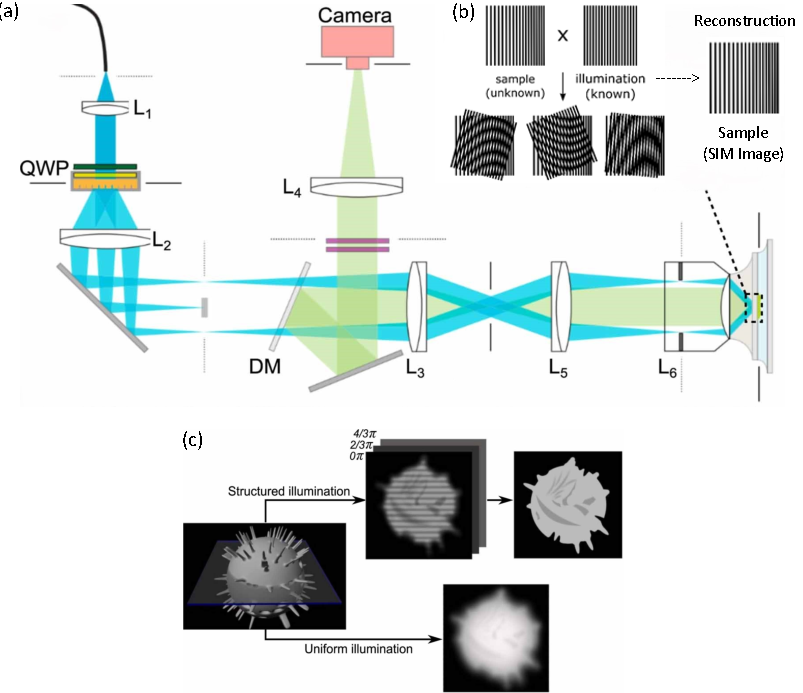
\includegraphics[width=\figwidth]{wide_filed_vs_SR_new.pdf}
	\slcaption{Adapted from \cite{microscope-picture} \cite{sim_image_reconstruction_adaptation}, the figure illustrates:
		(a) Schematic representation of the working principle of Structured Illumination Microscopy (SIM). 
		(b) Illustration of the moiré pattern generated through the interference of two coherent light beams,
		(c) Demonstration of how detailed information can be recovered using the SIM reconstruction algorithm from images modulated by the sinusoidal patterns in diffrent phase and angels.
		 \label{fig:wide_filed_vs_SR}}
\end{figure}
\vspace{1cm}
\noindent
\begin{figure}
	
	\centering
	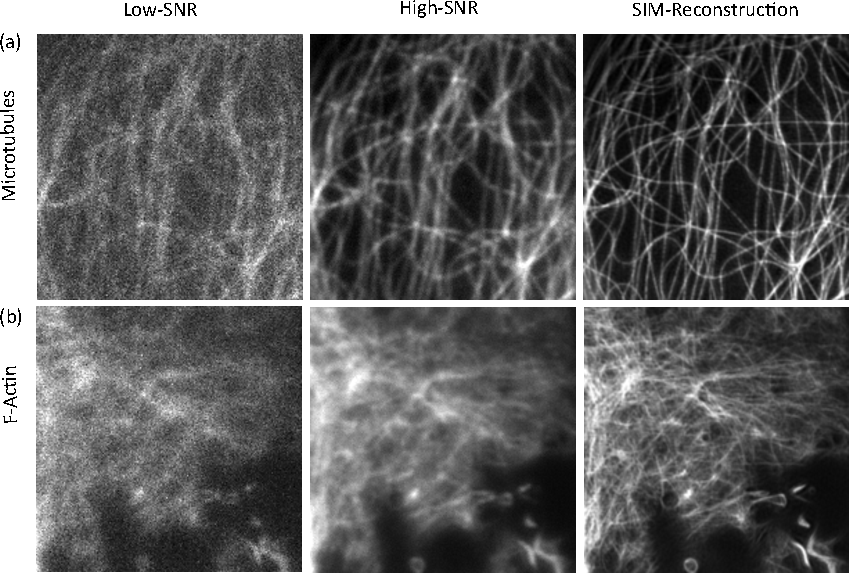
\includegraphics[width=1.0\linewidth]{mt_vs_fa_high_density.pdf}
	\slcaption{
		Wide-field images of Microtubules (a) and F-actin (b) under low-SNR (left) and high-SNR (middle) conditions, both limited by the Abbe diffraction limit, 
		are compared to the SIM-reconstructed super-resolution images (right) that achieve twice the classical resolution through reconstruction from pattern modulated data.
		 \label{fig:mt_vs_fa_high_density}}
\end{figure}
\vspace{1cm}
\noindent

%what is it, 
%how imaging works
%
\section{What is SIM Reconstruction? }

Structured Illumination Microscopy (SIM) reconstruction is an advanced computational technique designed to enhance image resolution beyond the diffraction 
limit of conventional light microscopy, which is approximately 200 nm laterally. In conventional microscopy, light emanating from a point source spreads 
out due to the point spread function (PSF), primarily because of diffraction. When two closely spaced objects emit light that is separated by less than the 
diffraction limit, their emitted light overlaps, resulting in a blurred region where the two objects are indistinguishable.


\vspace{1cm}
\noindent
SIM addresses this limitation by illuminating the specimen with a series of known, sinusoidal illumination patterns typically using three different angles 
and three different phases, as shows in \figref{fig:wide_filed_vs_SR} [b]. The sinusoidal illumination adds spatial frequency information to the object such that high frequency details, normally not 
observable due to the diffraction limit, are modulated into the lower frequency region of the image where they can be detected.


\vspace{1cm}
\noindent
Multiple raw images are acquired under these varying illumination conditions. A specialized reconstruction algorithm then processes these images to extract 
the high frequency information that was shifted into the observable frequency range during illumination. By combining this extracted information 
with the directly acquired low frequency content, the algorithm synthesizes a final image with enhanced resolution. Thus \figureref{fig:wide_filed_vs_SR} (c), the lateral resolution 
of the reconstructed image is roughly doubled compared to diffraction limited instruments, achieving a resolution in the range of approximately 100 nm, revealing the fine details of the object.



\subsection{FairSIM} 
\label{sec:fairsim}

FairSIM is a SIM Reconstruction plugin for Structural Illumination Microscopy for imageJ.
The SIM Reconstruction is performed numerically on the acquired widefield data from the microscope,
these algorithms allow to enhance the resolution by two fold in comparison with the corresponding acquired image. \cite{fairSIM}
This application can work on two beam interference, which is utilized by many home-built and total internal reflection-excited 
fluorescence (TIRF)-based systems. It is based on the well established SIM illumination technique introduced 
by Gustaffson and Heintzmann \cite{gustafson} \cite{heintzmann} , and the corresponding reconstruction algorithms.

\vspace{1cm}
\noindent
This application provides the biologist with the flexibility to approximate the parameter and the OTF automatically, 
with advance options to correct phase and angels of modulation, thus enhancing the reconstructed SIM image. 
The reliability of the SIM reconstruction and the user-friendliness makes it the preferred  choice for this project. 

\vspace{1cm}
\noindent

\section{Biological Specimens}

For the scope of this project, we focus only of 2 biological specimens, Microtubules and F-actin. 





\vspace{1cm}
\noindent


\subsection{Microtubules}
\label{sec:microtubules}
Microtubules are hollow, cylindrical repeating protein filaments formed by the assembly of alpha and beta tubulin heterodimers and are essential 
for maintaining cell architecture, intracellular transport, and mitotic spindle formation during cell division \cite{microtubules}. 
These rigid, hollow cylinders, about 25 nm in diameter, are made up of tubulin protein dimers that form long, spaghetti like filaments.
Unlike other cytoskeletal components, microtubules are relatively stable, yet they display dynamic instability at their ends, allowing 
rapid growth or shrinkage. In microscopy images, microtubules often appear as straight or curved lines emanating from the centrosome. 
The small diameter in nano meter and the overlapping filaments and sharpe edges makes is challenging of imaging and reconstruction of 
SIM images of this specific biological specimen. As shows in \figureref{fig:Structural_complexity} (a), the stractural complexity of microtubules(MT) 
has a large mean gradiant, proving it significantly challanging for image reconstruction tasks.


% if possible. inlcude an image





\vspace{1cm}
\noindent


\subsection{F-Actin}
\label{sec:f-actin}

F-actin, the filamentous polymer of globular actin (G actin) monomers, is a major component of the cytoskeleton that underpins cell shape, mobility, 
and force generation. The polymerization of G actin into F actin produces dynamic, polarized filaments with a rapidly growing “barbed” end and a slower
 “pointed” end that drive processes such as cell migration, endocytosis, and the formation of specialized structures (e.g., lamellipodia and filopodia)\cite{f-actin} . 
 The filamentous variant of actin comprises thin, flexible microfilaments approximately 7 nm in diameter that can extend several micrometers in length. 
The extreme nanoscale dimensions, overlapping filaments, and sharp edges, which can be easily lost by verly little noise, present significant challenges
for the imaging and reconstruction of SIM data for this biological specimen specifically for deep learning based methods. As shown 
in \figureref{fig:Structural_complexity} (a)
the stractural complexity of F-actin has a larger and wider mean gradiant then other specimen, which introduces by the complex and dense overlapping fillament, 
making it very difficult to sperate this fillament in image reconstruction tasks. The  \figureref{fig:mt_vs_fa_high_density} shows, the density and complexity of the F-actin filaments 
in the image and the SIM recons, compared with Microtubules. 


\section{Stcartural Complexity of different specimen}
\label{sec:structural_complexity}

The structural complexity measures the density and 
intricacy of a specific biological specimen. As presented in \cite{DFCAN}, for a given biological SIM image I, 
consisting of M × N pixels, its structural complexity is defined as its grayscale mean 
gradient (MG):

\begin{equation}
\label{eq:structural_complexity_eq}
MG(I) = \frac{1}{M \times N} \sum_{i=1}^{M} \sum_{j=1}^{N} \sqrt{\frac{ \left( \frac{\Delta I}{\Delta x} \right)_{ij}^{2} + \left( \frac{\Delta I}{\Delta y} \right)_{ij}^{2}}{2}}
\end{equation}


\vspace{1cm}
\noindent
Typical gradient maps and corresponding MGs of CCPs, ER, MTs and F-actin 
are shown in \cite{rdl_main}. For each type of biological specimen, 
we employed its mean MG (averaged from the MG scores of all its GT-SIM 
images in the BioSR dataset) to represent its structural complexity. As shown in \eqref{eq:structural_complexity_eq}, the structural complexity increases from punctate CCPs, 
reticular ER and string-like MTs to intricate F-actin.


\begin{figure}[H]
	\centering
	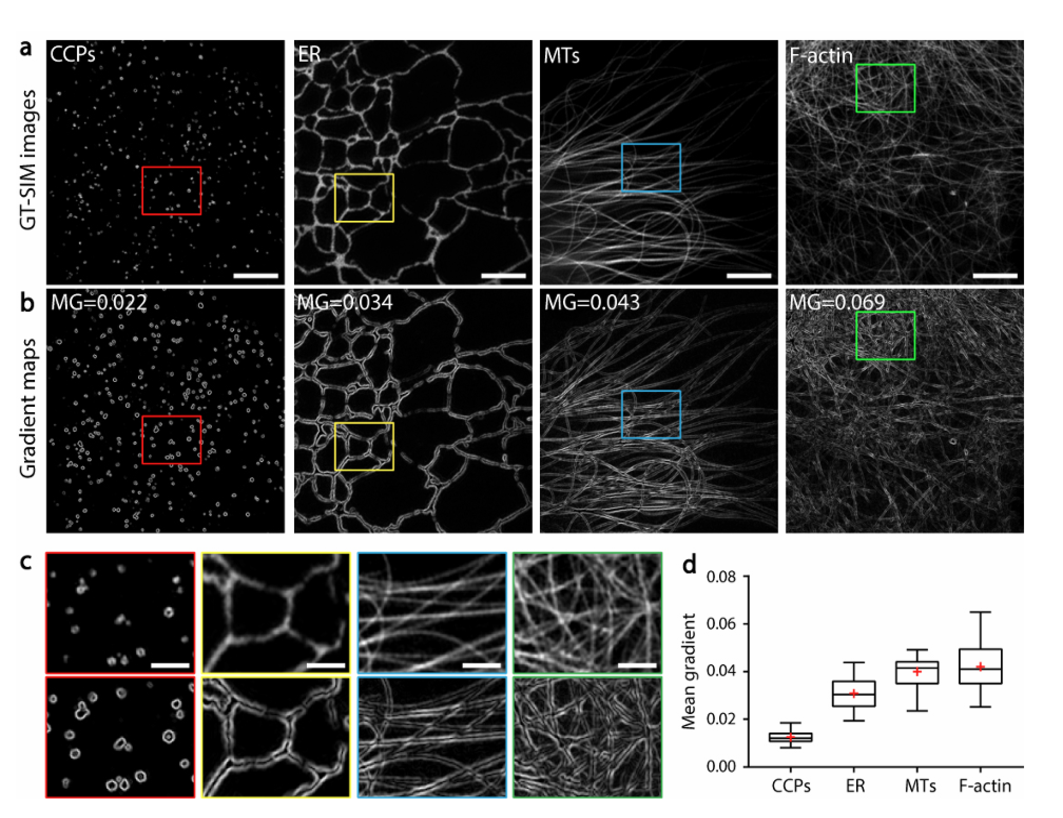
\includegraphics[width=\linewidth]{stractural-complexity.pdf}
	\slcaption{Assessment of structural complexity of different specimens with mean 
	gradient. (a), Representative GT-SIM images of CCPs, ER, MTs, and F-actin. (b) The corresponding 
	gradient maps to (a). (c) magnified images of the boxed regions from GT-SIM images (upper row) and 
	gradient maps (lower row). Scale bar: 3 $\mu$m (a), 1 $\mu$m (c). Experiments were repeated with more than 
	50 images, achieving similar results. d, Box-and-whisker plots of the mean gradients for CCPs (n=54), 
	ER (n=69), Microtubules (n=54) and F-actin (n=51). Central line, medians; red cross, mean; limits, 75\%
	and 25\%; whiskers, maximum and minimum. This illustration is taken from \cite{DFCAN} \label{fig:Structural_complexity}}
\end{figure}


\chapter{Methods}


\section{Deep Fourier Channel Attention Network (DFCAN)}
\label{sec:dfcan}


DFCAN is designed to improve image super-resolution from wide-field image to single super resoulation image. Instead of just working in the spatial domain of the image,
it also looks at the image in the fourier domain. This means it specifically examines the frequency data, where high frequencies are responsible for the fine details, 
like edges and textures. By focusing on these high-frequency components, DFCAN can restore more accurate details when converting low resolution images into super resoulation images.

\vspace{1cm}
\noindent
In this method, after extracting the high-level features with simple layer, it incorporates Fourier Channel Attention Blocks (FCAB),
that converts the features into frequency domain and calculates and enhances the power contribution of high-frequency components (the area that carries the fine details).
This extracted features are then carries out via skip connections keeping the low-frequency information details intact, which is followed by a pixel shuffle layer 
to  these feature blocks back into super resolution image. \cite{DFCAN}

\section{ScU-Net}
\label{sec:scu-net}
The U-Net architecture has significantly impacted the field of bioimaging since its introduction in May 2015. 
Its capability for feature localization and effective training on image patches has established it as a preferred method for image segmentation and reconstruction tasks.
The fundamental concept of U-Net involves enhancing a conventional contracting network by integrating successive layers, where standard pooling layers are substituted with upsampling layers.
This results in a U like shape, thus giving it the name U-Net. U-Net utilizes an increased number of feature channels in both the downsampling and upsampling part. Notably, at each downsampling step, 
the number of feature channels is doubled, optimizing the model's ability to capture intricate patterns. 
Furthermore, the architecture incorporates skip connections that transfer features from the 2D max-pooling segment to the 2D upsampling segment, 
thereby facilitating improved localization of features throughout the network \cite{U-net}.

\vspace{1cm}
\noindent
The scU-Net architecture take the idea further by chaining two 2D U-Nets together. 
This design addresses the limitations of a single U-Net, particularly regarding image reconstruction fidelity in 
low signal-to-noise ratio (SNR) conditions. By utilizing the output of the initial U-Net as input for the second U-Net, 
the architecture is trained against the ground truth, resulting in enhanced accuracy for reconstructing images affected
 by low signal to noise. This method demonstrates superiority over conventional Structured Illumination Microscopy (SIM) 
 reconstruction techniques, particularly under low-light conditions. \cite{Scu-net}
 

% \section{Rationalized Deep Learning Super-Resolution Microscopy (RDL-SIM)}
% \label{sec:rdl-sim}
% RDL-SIM is a deep learning-based super-resolution microscopy method that utilizes a convolutional neural network (CNN) to enhance the resolution of wide-field fluorescence images by incorporating prior knowledge of the modulation and illumination patterns used in structured illumination microscopy (SIM). For low signal-to-noise ratio (SNR) data, conventional SIM reconstruction is severely compromised by noise and artifacts, which this method addresses by denoising the input image prior to reconstruction.
% The idea behind it is, as a single U-Net suffer from image reconstruction fidelity from low signal to noise images,
% this image can be used as input for the chained U-Net and trained against the ground truth, which yield a more accurate result for noisy images 
% Compared with conventional SIM reconstruction under low-light conditions \cite{Scu-net}, the depth of the filter size in each convolution layer is doubled relative to the U-Net depth. 
% This design enables deeper layers to capture progressively more abstract features while preserving fine structural details, resulting in a more robust reconstruction even in challenging illumination scenarios.

\section{Rationalized Deep Learning Super-Resolution Microscopy (RDL-SIM)}
\label{sec:rdl-sim}
RDL-SIM is a deep learning-based super-resolution microscopy method that utilizes a convolutional neural network (CNN) to enhance the resolution of wide-field fluorescence 
images by incorporating the prior knowledge of the modulation and illumination patterns used in structured illumination microscopy (SIM).
For low signal-to-noise ratio (SNR) data, conventional SIM reconstruction is severely compromised by noise and artifacts. In this context, RDL-SIM leverages a neural network that 
is specifically trained to denoise low-SNR images while preserving the high-frequency illumination patterns inherent to SIM. By first applying this denoising procedure,
the subsequent SIM reconstruction algorithm operates on images with significantly improved SNR, thereby facilitating the extraction of high-resolution details.
The SIM reconstruction is performed on this denoised image can reconstruct high resoulation SIM image revealing detailed features, which was not possible by 
deep leaning based SIM reconstruction methods, directly from low-SNR data. \cite{rdl_main}

\vspace{1cm}
\noindent
The method introduced 3 brances of the 
network architecture, primary feature extraction (PFE) branch, Moiré Pattern Extraction (MPE) branch, and Feature Coalescing and Denoising (FCD) branch. 

\vspace{1cm}
\noindent

\subsection{primary feature extraction (PFE)}

The Primary Feature Extraction (PFE) branch is the first step in the RDL-SIM architecture, where it takes the noisy low-SNR wide-field image as input
and extracts the primary features. 



\subsection{Moiré Pattern Extraction (MPE) }

As the Moiré pattern has an important role in SIM reconstruction, the autor, characterized the illumination patterns and point spread function 
(PSF) of different SIM modalities under high SNR conditions. Because 
illumination patterns and PSF are natural attributes of the SIM system 
that are independent of observed specimens or available SNR levels 
of different experiments, these deterministic properties can be used 
to regulate the denoised raw images in compliance with the physical 
model of SIM \cite{rdl_main}. To Generate this pattern modulated images, the method depends on DFCAN, \sectionref{sec:dfcan},
calculates the modulation from the corrosponding high-SNR ground truth images, and then uses this as input for the MPE branch of the network.


\subsection{Feature Coalescing and denoising (FCD)}
In the brach, the features from the PFE and MPE branches are fused together to form a more comprehensive representation of the input image. 
The assumpotion is that the PFE branch captures the general features of the image, while the MPE branch focuses on the specific Moiré patterns.
By combining these two sources of information, the FCD branch aims to enhance the overall quality of the image reconstruction. 
The fused features are then processed through a series of convolutional layers to further refine and denoise the image. 
This denoising process is crucial for improving the signal-to-noise ratio (SNR) of the final output, making it more suitable for subsequent analysis and interpretation.
































\chapter{Image evaluation methods}
\label{sec:eval-metrics}

Quantification of performance for each network. To evaluate the reconstrued
images with the ground truth pair, we use various full reference image
measurement quality metrices, Such as MSE, NRMSE, PSNR, SSIM and MS-SSIM. Only
Decorrelation analysis is a parameter free resolution test that does not require
a reference image.

\subsection{Mean Squared Error}

MSE measures the average squared difference between pixel values of the ground truth and the predicted images. It is calculated as follows:

\vspace{1cm}
\noindent

\begin{equation}
\label{eq:MSE}
\text{MSE} = \frac{1}{N} \sum_{i=1}^{N} (y_i - \hat{y}_i)^2
\end{equation}

Where:

\begin{itemize}
	\item \(N\) is the number of pixels in the image.
	\item \(y_i\) is the pixel value of the ground truth image at pixel \(i\).
	\item \(\hat{y}_i\) is the pixel value of the predicted image at pixel \(i\).
\end{itemize}

\vspace{1cm}
\noindent
However, it has limitations in reflecting perceived visual quality, particularly for microscopy images rich in structural details,
as it focuses solely on pixel-wise differences. The lower the MSE value is, the better the image reconstruction. This Method is very sensitive
to Illumination and does not consider the underlaying characteristic of the image itself. MSE alone is not a good indicator of image reconstruction itself.



\subsection{Normalized Root Mean Square Error}
NRMSE enhances the Root Mean Squared Error (RMSE) by normalizing it with the image’s intensity range, enabling comparisons across datasets with similar scales.
It is expressed as:
\vspace{1cm}
\noindent


\begin{equation}
\label{eq:NRMSE}
\text{NRMSE} = \frac{\sqrt{\frac{1}{N} \sum_{i=1}^{N} (y_i - \hat{y}_i)^2}}{max(y) - min(y)}
\end{equation}

Where:

\begin{itemize}
	\item \(N\) is the number of pixels in the image.
	\item \(y_i\) is the pixel value of the ground truth image at pixel \(i\).
	\item \(\hat{y}_i\) is the pixel value of the predicted image at pixel \(i\).
	\item \(max(y)\) and \(min(y)\) are the maximum and minimum pixel values in the ground truth image, respectively.
\end{itemize}

\vspace{1cm}
\noindent

NRMSE is a more robust metric than MSE, as it accounts for the image’s intensity range, making it suitable for comparing images with different brightness levels.
is indeed useful for measuring shifts in pixel intensity because it directly compares the pixel values between two images. 
If the intensity of pixels changes (e.g., due to brightening, darkening, or other uniform shifts), 
this will increase the difference between $I_1(i)$ and $I_2(i)$, leading to a higher NRMSE. In this sense,
it effectively captures overall mismatches in pixel intensity across the image.

\vspace{1cm}
\noindent
However, when it comes to measuring how much structure has been shifted such as spatial rearrangements, 
translations, or distortions NRMSE has its limitations. As NRMSE used as a global metrics, it averages the error across all pixels, 
ignoring the spatial relationships between them. It only measures the magnitude of intensity differences, not their structural context.





\subsection{Peak Signal-to-Noise Ratio}


The PSNR is a signal processing measurement that compares a given
received or processed signal to its original source signal. This comparison
allows us to quantify how much a processed signal is faithful to the original,
also allowing us to identify possible noises or distortions to the signal. \cite{psnr-paper}
PSNR is a widely used metric to evaluate the quality of a processed image (e.g., reconstructed, compressed, or enhanced) 
compared to its original (ground truth) version. It measures the ratio of the maximum possible signal strength to the noise introduced by the processing, 
expressed in decibels (dB). Essentially, PSNR tells you how much distortion or noise is present in the processed image relative to the clean original.
Higher PSNR values indicate better image quality. 
PSNR is purely pixel-based and doesn’t account for how humans perceive quality. 
Two images with identical PSNR values might look very different if errors are distributed unevenly or affect perceptually important areas (e.g., edges in microscopy images).


\begin{equation}\label{eq:PSNR}
\text{PSNR} = 10 \cdot \log_{10}\!\left(\frac{\text{MAX}_{I}^2}{\text{MSE}}\right)
\end{equation}

where:
\begin{itemize}
	\item \(\text{MAX}_{I}\) is the maximum possible pixel value of the image (max(I)-min(I)).
	\item \(\text{MSE}\) is the mean squared error between the original and processed images.
\end{itemize}


\vspace{1cm}
\noindent
In the context of microscopy, PSNR is particularly effective for evaluating the fidelity of CNN-generated images in tasks such as denoising 
or super-resolution, where signal clarity is paramount \cite{CARE}. Higher PSNR is consider as better image reconstruction quality.This image evaluation method is 
purely pixel-based and doesn’t account for how humans perceive quality. Two images with identical PSNR values might look very different 
if errors are distributed unevenly or affect perceptually important areas (e.g., edges in microscopy images).


\subsection{Structural Similarity Index (SSIM)}

SSIM evaluates image quality by mimicking human visual perception, focusing on luminance, contrast, and structural similarities. \cite{ssim_paper} It is defined as:


\begin{equation}\label{eq:SSIM_general}
	\text{SSIM}(x, y) = l(x, y) \cdot c(x, y) \cdot s(x, y)
\end{equation}

Where:
\begin{itemize}
    \item \(l(x, y)\) is the luminance comparison function, quantifying the brightness similarity between images \(x\) and \(y\).
    \item \(c(x, y)\) is the contrast comparison function, measuring the contrast similarity of the two images.
    \item \(s(x, y)\) is the structure comparison function, evaluating the structural information contained within images \(x\) and \(y\).
\end{itemize}

The individual components of the SSIM can be articulated mathematically as follows:

\vspace{1cm}
\noindent


 1.  \textbf{ Luminance Function:}
\begin{equation}
	l(x, y) = \frac{2\mu_x\mu_y + C_1}{\mu_x^2 + \mu_y^2 + C_1}
\end{equation}
\begin{itemize}
  \item \(\mu_x\) and \(\mu_y\) denote the average pixel values of images \(x\) and \(y\), respectively.
  \item \(C_1\) is a constant introduced to mitigate the effect of weak denominators.
\end{itemize}

2. \textbf{Contrast Function}:
   \begin{equation}
   c(x, y) = \frac{2\sigma_x \sigma_y + C_2}{\sigma_x^2 + \sigma_y^2 + C_2}
   \end{equation}
\begin{itemize}
	\item \(\sigma_x^2\) represents the variance of image \(x\).
	\item \(\sigma_y^2\) represents the variance of image \(y\).
	\item \(C_2\) is an additional constant that stabilizes the division.
\end{itemize}

3. \textbf{Structure Function}:
\begin{equation}
	s(x, y) = \frac{\sigma_{xy} + C_3}{\sigma_x \sigma_y + C_3}
\end{equation}
\begin{itemize}
	 \item \(\sigma_{xy}\) indicates the covariance between images \(x\) and \(y\).
	 \item \(C_3\) is a constant that serves to prevent potential division by zero.
\end{itemize}
\noindent
The constants \(C_1\), \(C_2\), and \(C_3\) are critical for ensuring numerical stability, especially in cases where the denominators may approach zero. Typically, these constants are defined as follows:
\[
C_1 = (K_1L)^2, \quad C_2 = (K_2L)^2
\]
\begin{itemize}
	\item \(L\) denotes the dynamic range of the pixel values.
	\item The commonly used values for the constants are \(K_1 = 0.01\) and \(K_2 = 0.03\).
	\item These constants are established to mitigate issues related to numerical instability.
\end{itemize}


\vspace{1cm}
\noindent



SSIM evaluates how well the processed image preserves the visual structure of the original, considering human perception. 
It’s sensitive to distortions like blurring or artifacts that might not drastically change pixel values (and thus PSNR) 
but alter the image’s appearance. For example, A slightly blurred image might have a high PSNR (small pixel errors) but a 
lower SSIM due to lost structural detail. SSIM in measure between 0 and 1, where 1 is perfect similarity and 0 means no similarity at all. 
For CNN based reconstructed microscope images, SSIM can highlight how well structural details like, cell edges or tissue patterns are preserved, 
which is often more scientifically relevant than raw pixel accuracy. It complements PSNR by focusing on visual fidelity.



\subsection{Multi-Scale Structural Similarity Index (MS-SSIM)}



MS-SSIM address the limitation of SSIM and takes the idea even further.  
SSIM index algorithm introduced in \cite{ssim_paper} is a single-scale approach. 
MS-SSIM considers this drawback of the method because the right scale depends on viewing conditions (e.g., display resolution and viewing distance). 
MS-SSIM provides more flexibility than single-scale approach in incorporating the variations of image resolution and viewing conditions \cite{ms-ssim}. 
The overall MS-SSIM evaluation is obtained by combining the measurement at different scales using : 

\begin{equation}
\label{eq:MS-SSIM}
\text{MS-SSIM}(x, y) = \prod_{j=1}^{J} [l_j(x, y)]^{\alpha_j} \cdot [c_j(x, y)]^{\beta_j} \cdot [s_j(x, y)]^{\gamma_j}
\end{equation}

Where:
\begin{itemize}
	\item \(J\) is the number of scales.
	\item \(\alpha_j\), \(\beta_j\), and \(\gamma_j\) are the weights assigned to the luminance, contrast, and structure components at scale \(j\).
	\item The product is taken over all scales \(j\).
	\item The weights \(\alpha_j\), \(\beta_j\), and \(\gamma_j\) are typically chosen to sum to 1, ensuring that the overall MS-SSIM value is a weighted combination of the contributions from each scale.
	\item The weights can be adjusted based on the specific application or the characteristics of the images being compared.
\end{itemize}

\noindent
MS-SSIM is particularly useful in applications where images may be viewed at different scales or resolutions, such as in Biomedical imaging or remote sensing.


\subsection{Decorrelation Analysis}
\label{sec:decorrelation_analysis}



Decorrelation analysis assessing the resolution of individual super-resolved images based on image partial phase autocorrelation. 
The method is parameter free estimation and doe not require a reference image. The main algorithm is divided into 2 steps. 
Firstly, the algorithm compute the Fourier transform of an edge-apodized image, normalize it, and determine its Pearson correlation with the original image. 
In next step, the algorithm applies a variable-radius binary circular mask to the normalized transform and recalculate Pearson correlations 
to produce the resolution function d(r) .\cite{resolution_test} Which is calculated as follows:


\vspace{1cm}
\noindent

\begin{equation}
\label{eq:resolution}
	d(r) = \frac{\int \mathrm{Re}\{ I(k)I_n^*(k)M(k;r) \}\, dk_x\, dk_y}{\sqrt{\int |I(k)|^2\, dk_x\, dk_y \int |I_n(k)M(k;r)|^2\, dk_x\, dk_y}}
\end{equation}
	
	
Where:
\begin{itemize}
	\item \(I(k)\) is the Fourier transform of the image.
	\item \(I_n(k)\) is the Fourier transform of the normalized image.
	\item \(M(k;r)\) is the binary circular mask with radius \(r\).
	\item \(\mathrm{Re}\{\cdot\}\) denotes the real part of a complex number.
	\item \(*\) denotes the complex conjugate.
	\item \(dk_x\) and \(dk_y\) are the differential elements in the Fourier domain.

\end{itemize}


\vspace{1cm}
\noindent
We use the imageJ plugin of this application for calculating the resolution, we use the default parameter setting,
which are $N_r=50$ and $N_g=10$ with a radius of $r_{min}=0$ and $r_{max}=10$, as described in the basic user manual of the plugin. \cite{resolution_test}









\chapter{Projection Upsampling (PU) Network}
\label{sec:PU-Net_architecture}




\begin{figure}[H]
	\centering

	\hspace*{-1.5cm}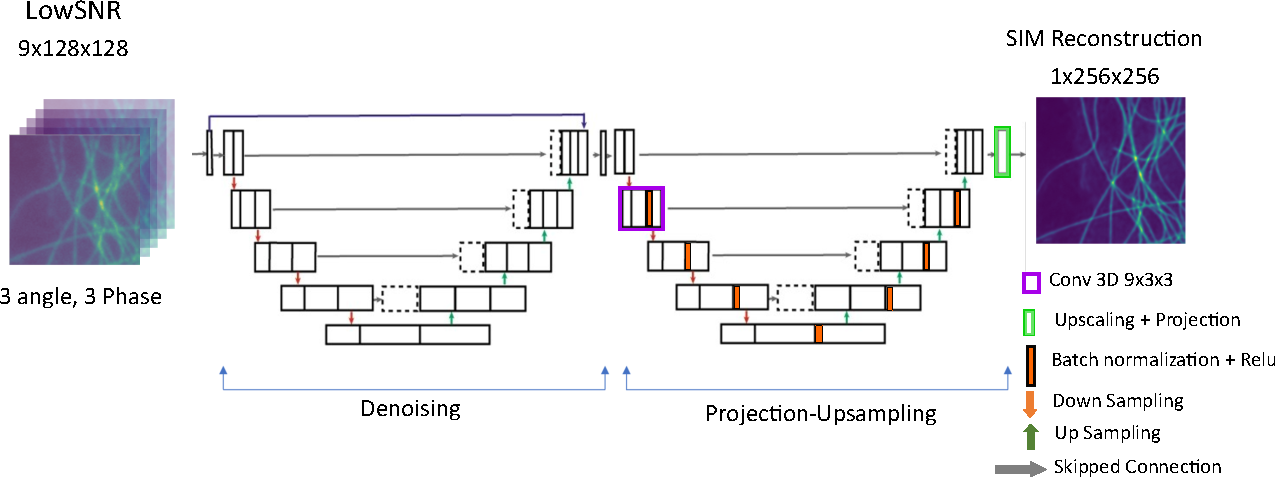
\includegraphics[width=1.2\textwidth]{PU-Net_explained.pdf}
	\slcaption{
		Illustrates the standard architecture of the Projection-Upsampling Network. Adapted from Figure 2 in \cite{Scu-net}, the framework integrates two 3D U-Net based architectures, followed by an upscaling block that aligns the network output with the ground truth. \label{fig:Scu-net}}
\end{figure}


In this study, we explore the potential benefits of employing three-dimensional kernels to capture spatial correlations along the channel dimension 
in the data from structured illumination microscopy. Conventional SIM typically excites specimens using sinusoidal illumination at various angles and phases,
 requiring acquisition of nine images (three angles, three phases) for two-beam SIM and fifteen images (three angles, five phases) for three-beam SIM 
 \cite{image_capture_in_microscopy}. Given that our imaging data and BioSR, both were acquired using a two-beam system, yielding nine-channel images,
  we hypothesized that treating the channel dimension as the z-axis in a three-dimensional convolutional framework might provide 
  additional spatial information beyond that captured by conventional two-dimensional kernels.


\vspace{1cm}
\noindent
To evaluate this hypothesis, we developed a Projection Upsampling (PU-Net) network that integrates two 3D U-Net architectures, 
linked by an upsampling layer, as illustrated in \figureref{fig:Scu-net}. In our experimental protocol, separate variants of PU-Net models
 were trained for each specimen types, Microtubules and F-actin. For each specimen, three PU-Net variants were implemented, 
 differing solely in the kernel size employed in the first initial layer of the chained U-Net architecture (purple block in the diagram) responsible for projecting 
 three-dimensional data to two dimensions. Specifically, for the first proejction layer the models utilized kernel sizes of 3x3x3, 7x5x5, and 9x3x3, respectively, 
 while all subsequent layers across PU-Net variants employed a standard 3x3x3 kernel. The network was trained and fine-tuned, with the parameters detailed in \tableref{tab:pu_net_summary}. 
 The loss function was chosen as the Mean Squared Error (MSE), based on our hypothesis that it would yield a considerably lower validation loss than the Mean Absolute Error (MAE), resulting into finner image reconstruction.


 





% Since the dataset consists of 9 channels , 3 angels, 3 phase and the speciman samples are stable, we sought out to see if we can utilize the learning ability of 3D kernals.
% The conventional SIM excites specimens with sinusoidal waves at different angels and phases.  Typically, it requires 9-images (3 angles, 3 phases) for two-beam SIM and
% 15 images (3 angles, 5 phases) for three-beam SIM \cite{image_capture_in_microscopy}. As the imaging data we uses comes from 2 beam system, 
% producing 9 channel images, we sought out to see, if capturing spatial correlations across the channel dimension by considering it as z-axis, if it could add more information that is not present in 2D kernels.
% in our experiment, the Projection Up sampling network consists of combining two 3D U-Net architecture combined together with an umsampling layer, as swown in \figureref{fig:Scu-net}.  
 

% % Write your paragraph here.
% \vspace{1cm}
% In our experiment, we train 3 PU-Net for each specimen, microtubules and F-actin separately. For each PU-Net experiment, we use 3 different kernel size for the first 
% layer only on the chained U-Net architecture for projection of 3D to 2D image data. We use kernel size of 3x3x3 for PU-Net (3x3x3), kernel size of 7x5x5 for PU-Net (7x5x5) 
% and kernel size of 9x3x3 for PU-Net (9x3x3). Further down the network, all the PU-Net variant uses kernel size of 3x3x3. We use MSE  as presented in equation \eqref{eq:MSE}, as loss function and fine tune the parameters 
% of network for each specimen for finer image reconstruction. \tableref{tab:pu_net_summary} summarizes the different PU-Net variants used in our experiments.


\section{Training Details}
In Projection-Upsampling Network, or in short PU-Net experiments, we utilized a mix of samples from  various low-light conditions of single specimen, with an input patch size of 
128×128×9  with a corresponding ground truth SIM reconstruction derived from hign SNR data, with patch pair of the input data sized at 
256×256×1. The final layer of our PU-Net incorporates an upscaling layer designed to increase the shape of the output to match that of the ground truth. Each Conv 3D layer is followed by Kernel Regularizer, Batch Normalization layer and ReLU activation function (see  \figureref{fig:Scu-net} orange block).	
The network is trained using the stochastic gradient descent, Adam optimizer with a $\beta_1$ of 0.9 and $\beta_2$ of 0.999. The step size is set of the mini batch ittareation is determined by number of training sample size divided by batch size. 
The augmentation piepeline makes sure the netwrok sees slightly different variation of the input data in each batch to make the learning process more effective. 

\vspace{1cm}
\noindent
To determine the optimal training parameters, we conduct parameter sweeps across different combinations, observing the significance of these parameters in relation to the loss curve. 
The training parameters are documented in \tableref{tab:pu_net_summary}. Our experiments we used both Mean Square Error (MSE) and Mean Absolute Error (MAE) as loss functions. The loss fucntion for our training experiment is defined as 






\begin{equation}\label{eq:MSE}
\text{MSE} = \frac{1}{H \times W \times Z} \sum_{i=1}^{H} \sum_{j=1}^{W} \sum_{k=1}^{Z} \left(y_{ijk} - \hat{y}_{ijk}\right)^2
\end{equation}

\vspace{1cm}

\begin{equation}\label{eq:MAE}
\text{MAE} = \frac{1}{H \times W \times Z} \sum_{i=1}^{H} \sum_{j=1}^{W} \sum_{k=1}^{Z} \left| y_{ijk} - \hat{y}_{ijk} \right|
\end{equation}

\begin{itemize}
    \item \(H \) is the height of the input .
    \item \(W \) is the width of the input.
    \item \(Z \) is the depth of the input.
    \item \(y_{ijk}\) is the ground truth  \((i,j,k)\).
    \item \(\hat{y}_{ijk}\) is the prediction  \((i,j,k)\).
\end{itemize}

\vspace{1cm}
\noindent
Ultimately, our experiments confirmed that minimizing the MSE during training not only improved the reconstruction fidelity 
but also yielded a lower validation loss, thereby enhancing the model's overall performance in reconstructing ground truth data from noisy input images.



\subsection{Data Generation and Augmentation}
For training, we use BioSR dataset \cite{BioSR}, which consist of Microtubules in 9 different signal to noise level and F-actin on 12 signal to noise level and their corresponding GT-SIM image. 
For generating the training data we mix all 9 noise level for Microtubules and 8 different noise level for F-actin dataset. 
We select 40 randomly selected image cells for training data generation, 7 for validation and 5 for testing. 
Form each image cell we create patch of 128x128x9 from different region of image with a total number of ~15000 image patches for training and ~4500 image patches for validation. 
While creating the image patches, we keep the select the regions with no-background information to make sure the network train on image patches where maximum information is available. 

\vspace{1cm}
\noindent
As very little training data available in BioSR dataset for each specimen of cells, we relay on heavy image augmentation. As in Biomedical imaging, deformation and rotation are the most 
common variations, we rely on different affine transformation of data, random crops and scaling. The data augmentation optimizes the network for desired invariances thus making it robust 
in hyperplanes. The necessity of data augmentation for learning invariances has been well experimented in Dosovitskiy et al \cite{augmentation_hyperplane}. Moreover, to make sure network learns the features more robustly, 
instead of doing the data augmentation when generating the training data, we use Data Wrapper function inside the training function to  create augmented data for each batch on the fly. 
This makes sure that in each batch, the network sees the augmented variation of the same data, thus making the training process more effective. 

% End of Data Pre-processing subchapter.

\subsection{Image Normaliaztion and Background Filtering}
\label{sec:image_normalization}



Image normalization and background filtering are critical pre-processing steps in the generation of eligible training data from microscopic images, 
ensuring consistency in intensity levels across samples and improving overall model performance. 

\vspace{1cm}
\noindent
For normalization, we use a percentile-based approach that adjusts image intensity using $p_{low} \in (1,3)$ and $p_{high} \in (99.5,99.9)$ thereby ensuring 
robust normalization that reduces the influence of outliers and hot spots commonly  known in microscopy image,  while preserving the essential structure of the image data.


\vspace{1cm}
\noindent
Background content in training images can negatively affect the learning process by introducing unwanted distributions. 
To eliminate this issue, image patches containing excessive background are systematically excluded from the training dataset. We implement 
a selection criterion whereby patches are considered eligible only if they meet a background threshold of 0.4. This threshold is applied in conjunction
with a maximum filter, which is used to identify and retain regions exhibiting the highest intensity values within the image sample. The integration of these
techniques facilitates the extraction of informative image patches that are less contaminated by background noise, thereby enhancing the quality of the training data.








\vspace{1cm}

\begin{table}[ht]
	\centering
	\caption{Summary of Pu-Net variants applied to the MT and F-actin datasets.}
	\label{tab:pu_net_summary}
	\resizebox{\textwidth}{!}{%
	\begin{tabular}{l c c c c c c}
		\toprule
		Parameter &
			\shortstack{PU-Net\\(3x3x3)} &
			\shortstack{PU-Net\\(7x5x5)} &
			\shortstack{PU-Net\\(9x3x3)} &
			\shortstack{PU-Net\\(3x3x3)} &
			\shortstack{PU-Net\\(7x5x5)} &
			\shortstack{PU-Net\\(9x3x3)} \\
		\midrule
		Dataset                   & MT      & MT      & MT      & F-actin & F-actin & F-actin \\
		Patch Size                & 128x128x9 & 128x128x9 & 128x128x9 & 128x128x9 & 128x128x9 & 128x128x9 \\
		U-Net Depth               & 4       & 2       & 3       & 4       & 2       & 4      \\
		U-Net First (filters)     & 64      & 48      & 32      & 64      & 48      & 64     \\
		U-Net Kernel              & 3       & 3       & 3       & 3       & 3       & 3      \\
		Residual Block            & True    & True    & True    & True    & True    & True   \\
		Proj. Kernel (1st-layer)  & 3x3x3   & 7x5x5   & 9x3x3   & 3x3x3   & 7x5x5   & 9x3x3  \\
		Proj. Kernel (block)      & 3x3x3   & 3x3x3   & 3x3x3   & 3x3x3   & 3x3x3   & 3x3x3  \\
		Proj. Depth               & 3       & 2       & 2       & 3       & 2       & 2      \\
		Proj. Conv/Depth          & 2       & 3       & 2       & 2       & 3       & 3      \\
		Batch Size                & 16      & 32      & 16      & 16      & 32      & 128    \\
		Learning Rate             & 0.0004  & 0.004   & 0.0004  & 0.0004  & 0.004   & 0.0004 \\
		Upsampling Factor         & 2       & 2       & 2       & 2       & 2       & 2      \\
		Loss Function             & MSE     & MSE     & MSE     & MSE     & MSE     & MSE    \\
		Batch Norm                & True    & True    & True    & True    & True    & True   \\
		Kernel Regularizer        & $l_2(0.0003)$ & $l_2(0.0003)$ & $l_2(0.0003)$ & $l_2(0.0003)$ & $l_2(0.0003)$ & $l_2(0.0003)$ \\
		Total Params.             & 22,068,354 & 1,749,938  & 1,485,506  & 22,068,354 & 1,749,938 & 38,010,686 \\
		\bottomrule
	\end{tabular}%
	}
\end{table}

\section{SIM Reconstruction result analysis}






% mt results
\begin{figure}[H]
	\centering
	\hspace*{-1cm}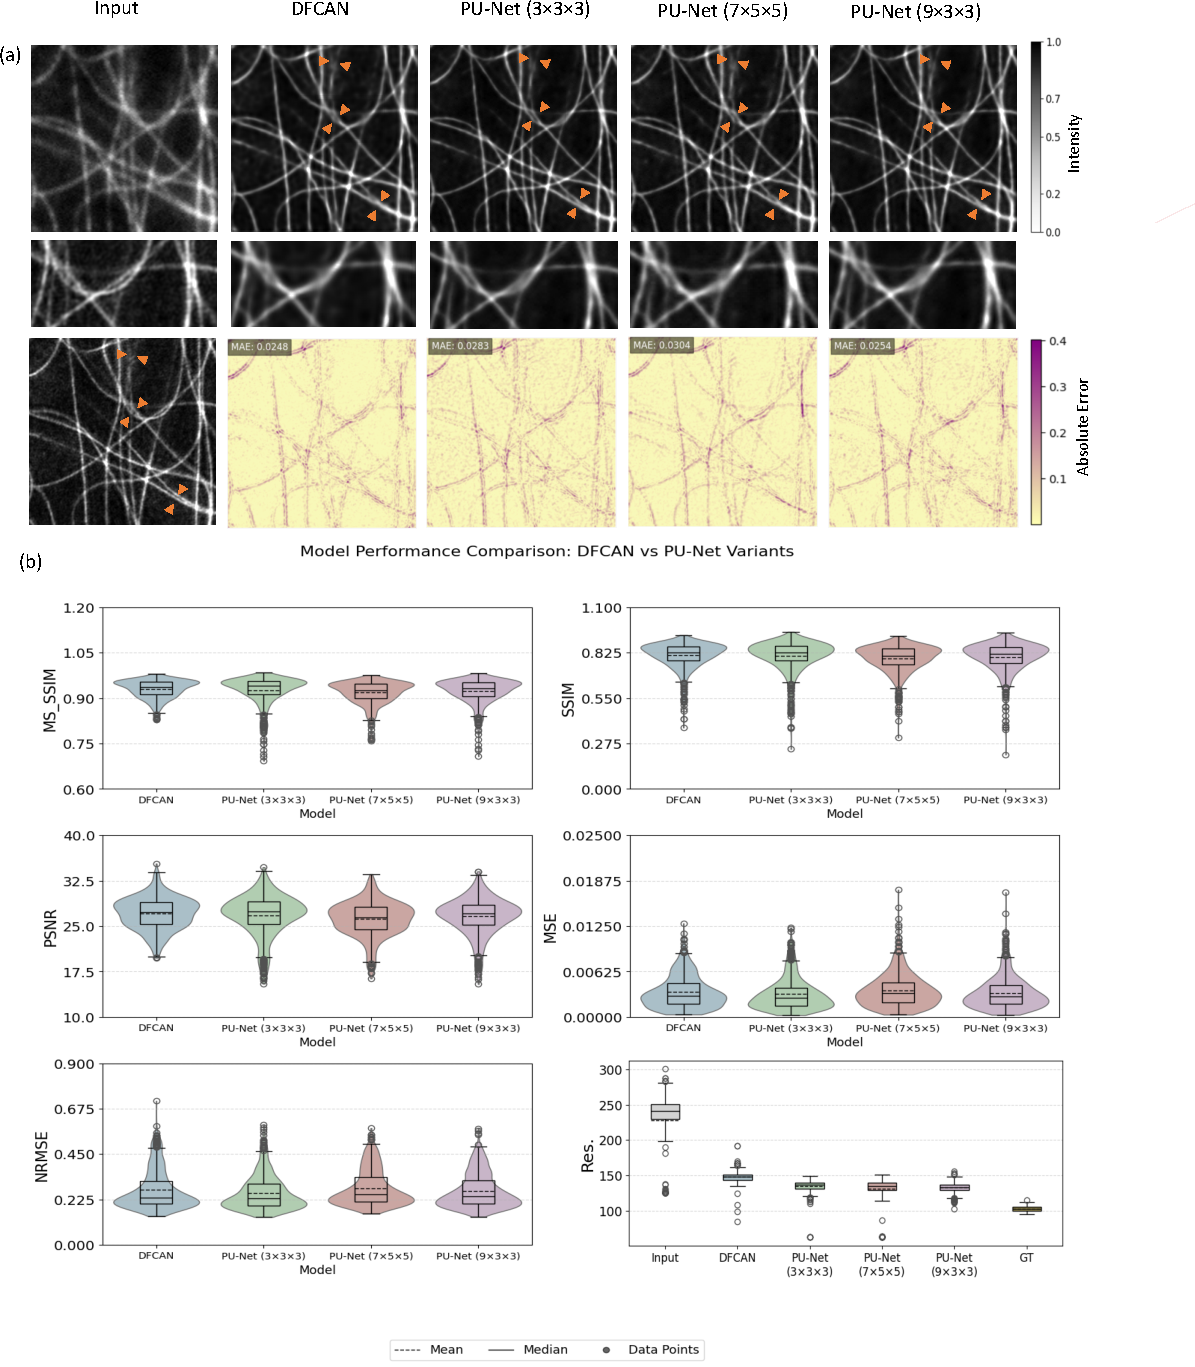
\includegraphics[width=\textwidth]{MT_SR_U_NET_COMPARISION_resized_new.pdf}
	% ensure there is enough space for the caption (adjust the required space as needed)
	% \needspace{1\baselineskip} 
	\slcaption{
		(a) A qualitative analysis of SIM reconstructions for Microtubules generated by DFCAN and various PU-Net (3×3×3, 7×5×5, and 9×3×3)
		is presented. The arrows indicates regions where the network prediction shows differences from both DFCAN and PU-Net variants.
		 
		(b) A statistical evaluation of the DFCAN and PU-Net model variants reveals comparable performance between the two approaches
		in SSIM and NRMSE. However, the resolution analysis indicates that PU-Net exhibits a considerable
		improvement in resolution.
		\label{fig:Mt_SR_U_NET_COMPARISION_resized}
	}
\end{figure}

% mt errors

\begin{figure}[H]
	\centering
	
	\hspace*{-1cm}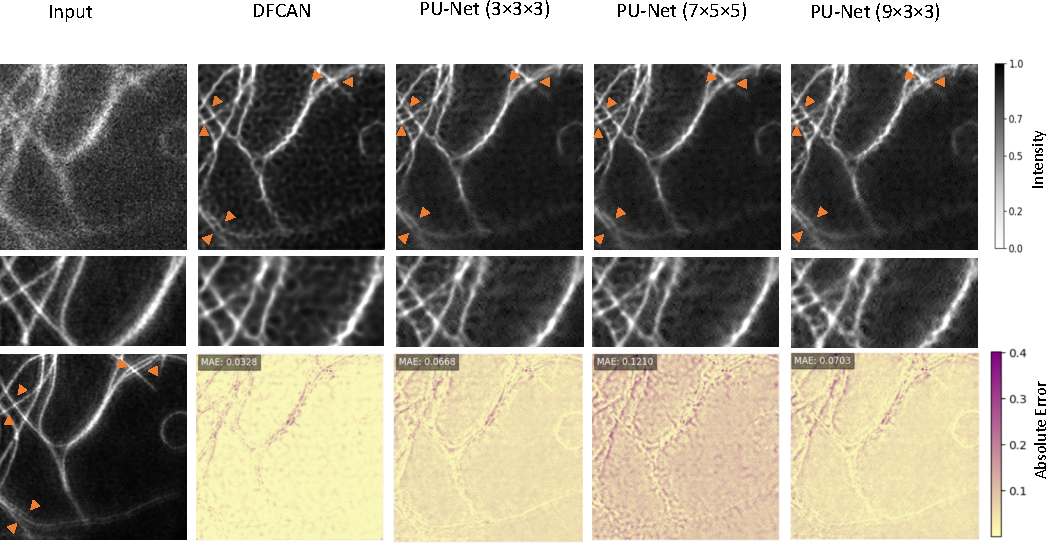
\includegraphics[width=\textwidth]{Mt_error_sim_recon_new.pdf}
	\slcaption{ 
		The network prediction from low-SNR Microtubules data presents significant challanegs in accurately reconstructing the ground truth data. Artifacts are evident across all approaches,
		  highlighting difficulties in maintaining image fidelity.
		  \label{fig:MT_error_sim_recon}}
\end{figure}
% factin results


\begin{figure}[H]
	\centering

	\hspace*{-1cm}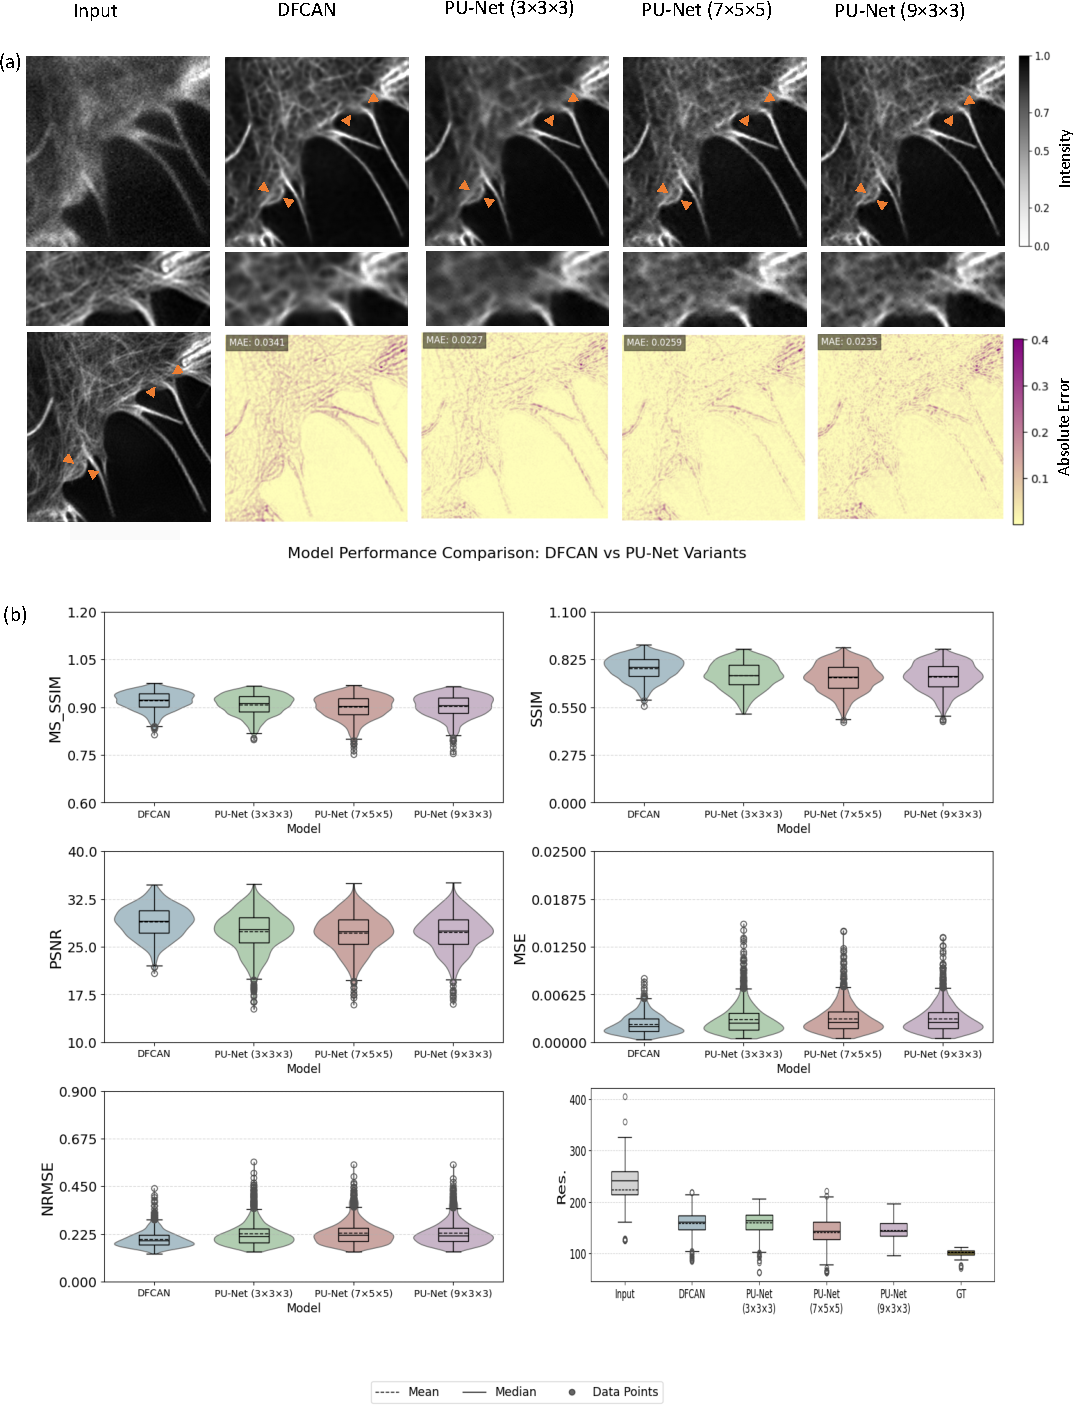
\includegraphics[width=\textwidth]{FT-sr-u-net_new.pdf}
	\slcaption{
		(a) The network prediction form DFCAN and  PU-Net configurations with the notable differences pointed by the arrow, demonstracteds the fedility in reconstruction. 
		(b) A statistical evaluation of the DFCAN and PU-Net model variants demonstrates on F-actin dataset.The resolution analysis indicates that enhancemenet in PU-Net (9x3x3) image resolution

		\label{fig:FT-sr-u-net}}

\end{figure}


% factin errors

\begin{figure}[H]
	\centering

	\hspace*{-1cm}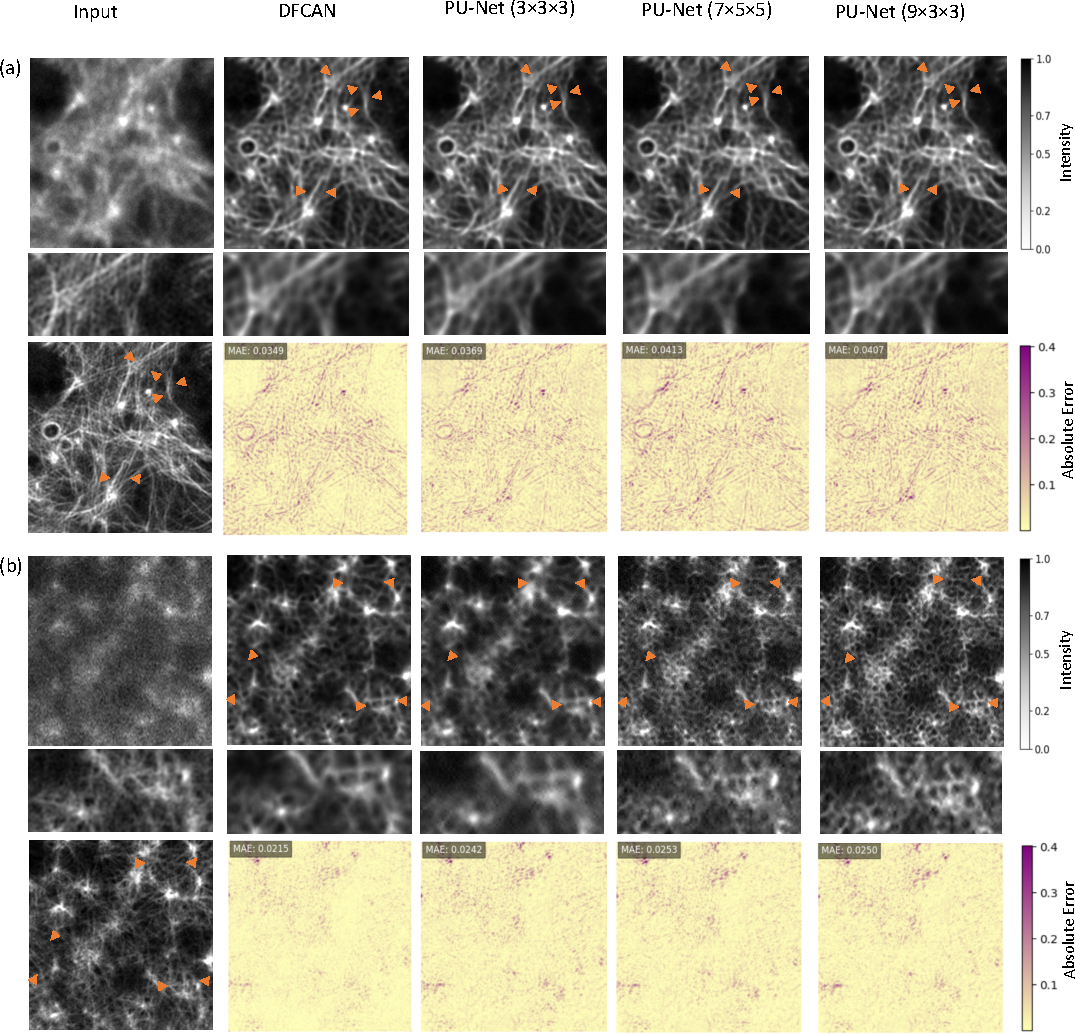
\includegraphics[width=\textwidth]{FA-errors_NEW.pdf}
	\slcaption{
		(a) SIM reconstruction of F-actin from medium signal-to-noise ratio (SNR) raw data indicates that both DFCAN and PU-Net
		 variants demonstrate comparable reconstruction capabilities. 

		 (b) In contrast, for low-SNR data, where the structures are severely noisy, 
		 PU-Net (7×5×5) and PU-Net (9×3×3) exhibit a distinct advantage over DFCAN in capturing spatial correlations across the channel dimension.




	\label{fig:FA-errors}}
\end{figure}
% uni results

\begin{figure}[H]
	\centering
	
	\hspace*{-1cm}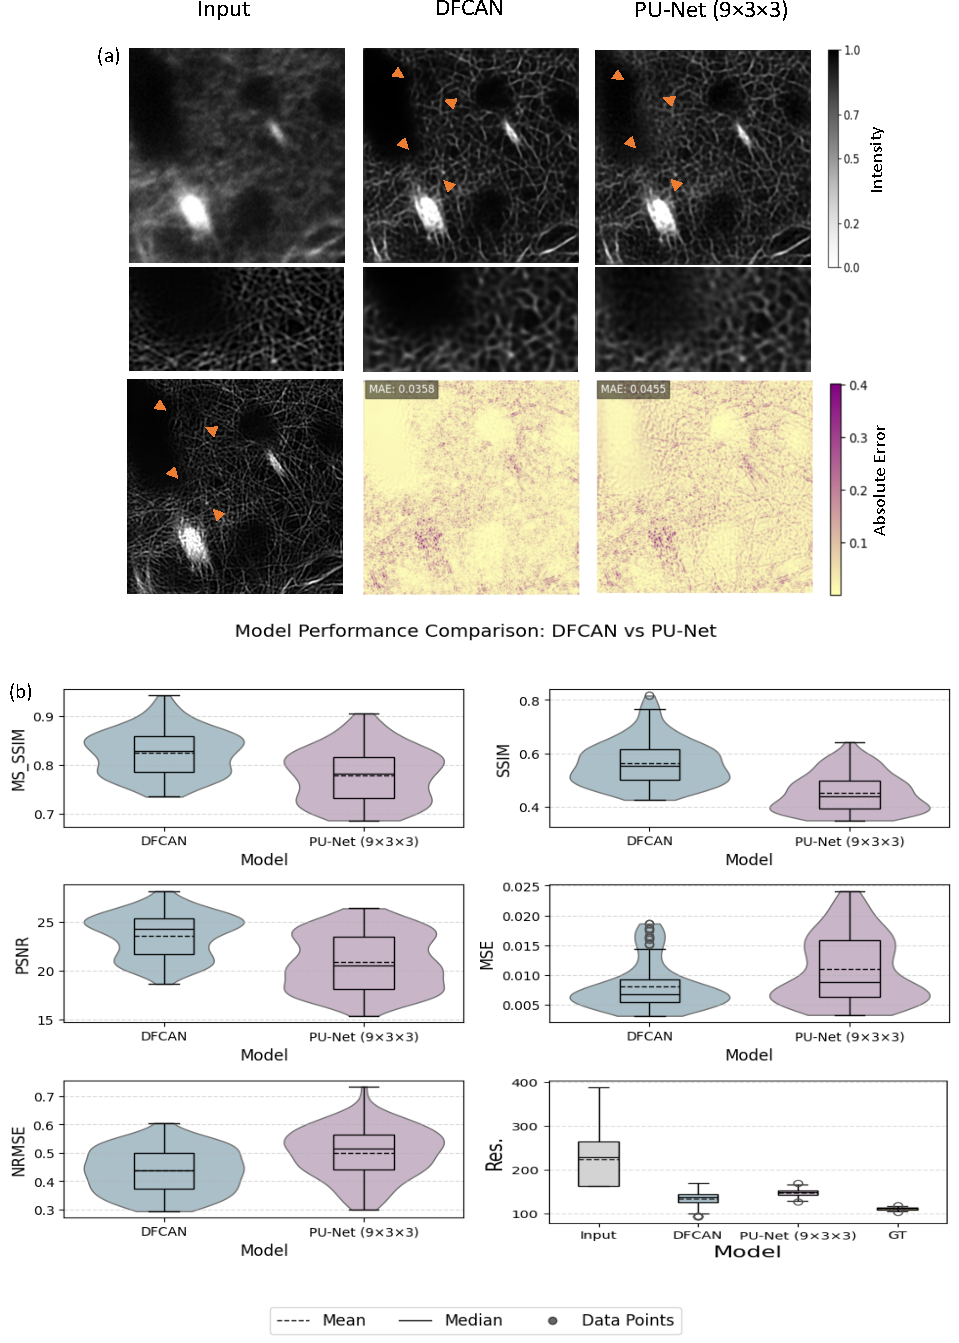
\includegraphics[width=\textwidth]{Uni_data_comparision_NEW.pdf}
	\slcaption{
		(a) Presents the network output from our own F-actin dataset, where we can observe that (orange marks) the PU-Net (9×3×3) captures more information then DFCAN.	
		(b) The bimodal distribution of the evaluation metricies indicates challanges generlization by the model on the valication data. 
		\label{fig:Uni_data_comparision}}
\end{figure}

\subsection{Microtubules analysis}
\label{sec:microtubules_analysis}

% In our experiments, we evaluate the performace of Microtubules dataset trainig with DFCAn and differnet PU-Net variants. As presented in \figref{fig:Mt_SR_U_NET_COMPARISION_resized}, marked with orange arraw, we can see that 
% PU-Net can reconstruct detailed features of the fillamnet, where DFCAN fails to distinguish the features. This is further evident in teh resolution analysis, where PU-Net varint shows better resolution than DFCAN.

% \vspace{1cm}
% \noindent
% Note that, for bvery noisy data, all the network prediction suffers from artifacts, as shown in \figref{fig:MT_error_sim_recon}, which failed to generate any sensible decorrelation analysis. For this reason, in the resolution analysis, 
% we only consider image that has higher resolution then 95nm achived by PU-Net (9x3x3) to compare the model predictions. 

In our experiments, we evaluate the performance of the Microtubules with DFCAN and various PU-Net variants. 
As illustrated in \figref{fig:Mt_SR_U_NET_COMPARISION_resized}, indicated by the orange arrow, PU-Net is able to reconstruct detailed 
features of the filament more effectively, whereas DFCAN fails to distinguish these features. This observation is further supported by the resolution 
analysis, where the PU-Net variant demonstrates notably higher resolution compared to DFCAN.

\vspace{1cm}
\noindent 
It is important to note that for highly noisy data, all network predictions are subject to artifacts, as depicted in \figref{fig:MT_error_sim_recon}, 
which failed to yield a meaningful decorrelation analysis. Consequently, in the resolution evaluation, we restrict our comparison to images with a resolution 
exceeding 95 nm, as achieved by PU-Net (9x3x3), to ensure a fair and reliable assessment of the model predictions.



\subsection{F-actin analysis}

% For F-actin, the dataset is much more challanginf then microtubules due to its dense mesh structure and increadabily smaller fillaments. From out experiment, we observe that, \figureref{fig:FT-sr-u-net} (a) show that, PU-Net (9x3x3)
% captures more detailed infromation then Pu-Net (3x3x3) or DFCAN. This is also evident in the resolution analysis, where PU-Net (9x3x3) shows better resolution then DFCAN and PU-Net (3x3x3).
% This is possbile beacuse the Pu-Net (9x3x3) is able to capture the spatial correlation across the all channel dimension, which is not possible with DFCAN, which utilizes 2D Conv layers or PU-Net (3x3x3).

For F-actin, the dataset poses greater challenges compared to microtubules due to its dense network structure and much smaller filament dimensions. Our experiments reveal that, as illustrated in \figureref{fig:FT-sr-u-net} (a),
 the PU-Net (9×3×3) architecture captures finer structural details than both PU-Net (3×3×3) and DFCAN. This finding is further substantiated by the resolution analysis, which demonstrates that PU-Net (9×3×3) 
 achieves higher resolution compared to the other models. This enhanced performance can be attributed to its ability to capture spatial correlations across all channel dimensions of Pu-Net (9x3x3), a capability that is limited 
 in DFCAN (which employs 2D convolutional layers) and PU-Net (3×3×3).

% For very noisy data, the limitation of all the approaches is evident in \figureref{fig:FA-errors} (a), where the network prediction from low-SNR data shows that, it significantly struggles to generate fine details present in the ground truth data.
% This challages can be mitigated by having more traininf data sample, so that the newtrok can learn to generalize and reconstructed the exceptional finner diteals. 
\vspace{1cm}
\noindent
Moreover, for extremely noisy and very dense data, all approaches exhibit limitations, as evidenced in \figureref{fig:FA-errors} (a), 
where network predictions derived from low-SNR data struggle to reproduce the fine details evident in the ground truth. 
This challenge may be mitigated by increasing the volume of training samples, thereby enabling the network to better generalize and reconstruct the intricate features.

% Fothermore, we test the netwrok with out own F-actin dataset, where we observe a bimdal distribution of the evaluation metrics, as shown in \figureref{fig:Uni_data_comparision} (b).
% This indicates the limitaion of training data, being small and less variationfor each stracture presented. This is evident in validation dataset set as well from the metricies. This gives us an important inside on our training data generation, 
% where we need to have more variation of the training data, so that the network can learn to generalize and reconstruct the finer details.
% \vspace{1cm}
\vspace{1cm}
\noindent
Furthermore, when testing the network on our own F-actin dataset, we observed a bimodal distribution in the evaluation metrics, as shown in \figureref{fig:Uni_data_comparision} (b). This suggests a limitation in the training data, which is relatively small and exhibits 
limited variation among the presented structures. A similar trend is observed in the validation dataset. These findings underscore the need for a broader 
and more diverse training dataset, which would facilitate improved generalization and finer detail reconstruction by the network.











\chapter{Denoising low-SNR data} 
Analyzing the denoising and SIM reconstruction in complex biological specimens such as F-actin presents several challenges,
due to its nature of complex overlapping mash stracture and high density. 


\vspace{1cm}
\noindent
In our work, we take the approch of RDL-SIM \cite{rdl_main}, as described in \sectionref{sec:rdl-sim}.
This technique first generates a SIM reconstruction image via DFCAN, after which a pattern-modulated image is computed from the reconstructed SIM image. 
The pattern-modulated image, together with the corresponding raw noisy image data, is then used as input to the network to generate a high signal-to-noise ratio (high-SNR) image. 
The resulting high-SNR image is subsequently post-processed using fairSIM  \sectionref{sec:fairsim} to produce the final SIM reconstruction.



\vspace{1cm}
\noindent
In our modified approach, we investigate the potential of exploiting the spatio temporal correlations captured by the z-dimension in the 3D kernel 
of PU-Net (9×3×3), as detailed in section \sectionref{sec:PU-Net_architecture} replacing the DFCAN model in the original training pipeline of RDL-SIM.
This substitution is designed to determine whether PU-Net can effectively generate the pattern-modulated image from the initially reconstructed SIM image, 
and to evaluate its impact on the quality of the subsequently denoised high-SNR image and the resultant SIM reconstruction.




\section{Data geneartion}
\label{sec:data-generation}
For the training the models on differnet biological specimans seperately, we produce 2 different training dataset for each speciman of low and 
mid SNR levels with respect to its high SNR data. We divide our training data as 40 cells for trainfing, 7 cells for validation and 6 cells for testing randomly. 
For training, from each cell we create 128x128x9 patches from different regions of the image, thrashholder by background of 0.4, futher augmented by random 
flip, rotation and translation, producing ~5500 patches for training. The dataset has been further normalized as described 
in \sectionref{sec:image_normalization}.



\section{Trainig details of rdl SIM}
\label{sec:training-details-rdl-sim}

In this work, we train the rdl-SIM model using the same training protocol outlined in \cite{rdl_main}. 
Specifically, the training is conducted with a batch size of 3, a relu coefficient of 0.1, and a learning rate of 0.0001. 
The depths of the branches are set accordingly, while the parameters for moiré pattern extraction (MPE), primary 
feature extraction (PFE) and feature coalescing and denoising (FCD) are assigned values of 5, 2, and 5, respectively. 
The loss function utilized is a composite of 
the mean squared error (MSE) and the structural similarity index measure (SSIM), weighted by a factor of 0.1. Under 
these conditions, we perform two experiments for each specimen by replacing the original SIM reconstruction module 
based on DFCAN with a PU-Net configuration (9×3×3). For the analysis of the result, we use 2 different biological specimen,
 Microtubules and F-actin from BioSR dataset \cite{BioSR}.

 \vspace{1cm}
\noindent
 In our experiments, we evaluate the performance of our proposed training pipeline using 2 different biological specimen datasets 
 under varying SNR conditions. Specifically, for the Microtubules dataset, each network—DFCAN + RDL and PU-Net (9×3×3) + RDL is 
 trained using either low-SNR or mid-SNR raw data as inputs, with the corresponding high-SNR raw data serving as the ground truth. 
 Similarly, for the F-actin dataset, separate networks are trained for low-SNR and mid-SNR inputs, again using high-SNR raw data as 
 the ground truth. This unified approach across different specimens facilitates a comprehensive comparison of network performance under diverse noise conditions.




% \section{Results Analysis of RDL SIM}

% In this section, we present the results of our RDL-SIM experiments from the BioSR dataset \cite{BioSR}.
% We compare the performance of the DFCAN + RDL and PU-Net (9×3×3) + RDL approaches,
% which are trained on low-SNR and mid-SNR raw data, respectively.

% For Mictorubules, we use 2 different SNR levels, low-SNR and mid-SNR. For both SNR levels,
%  we observe that the DFCAN + RDL and PU-Net (9×3×3) + RDL approaches yield similar results for both low-SNR 
%  \figref{fig:MT-02_DN-Compariosin} and mid-SNR data\figref{fig:Mt-04_DN}
%  in terms of image reconstruction and evaluation metrics. This is also evident in the image reconstruction, 
% where both approaches yield comparable results in SIM reconstruction achived by FairSIM \sectionref{sec:fairsim} plugn in Imagej.

% \vspace{1cm}
% For F-actin, we also use 2 different SNR levels, low-SNR and mid-SNR.
%  For low SNR levels, we observe that the DFCAN + RDL and PU-Net (9×3×3) + RDL approaches yield similar results 
%  in terms of image reconstruction and evaluation metrics. However, the reconstruction of fine filament details
%   is challenging for both approaches,as shwon in figure \figref{fig:FA-DN_04} (a) with fairSIM plugin, where it struggels to find paramters,  
%   suggesting that, the small training data and the high structural density of the data are the major challages. Tthis can be seen in the
%   evaluation metrics \figref{fig:FA-DN_04} (b) where the NRMSE and MSE where the distribution is wider suggesting the model is 
%   struggling to generalize the fine details features. 


%   \vspace{1cm}
%   Howver, for mid-SNR levels, we observe that the image reconstructions are close to the High-SNR data. This is also evident in 
%   SIM reconstruction via FairSIM \sectionref{sec:fairsim} plugn in Imagej, presented in \figref{fig:FN-08_DN_comparision} (a). The both SIM reconstruction exhibits similar performance, 
%   comparable to the high SNR SIM reconstruction where fine filament details are well reconstructed. The quantification metricies in \figref{fig:FN-08_DN_comparision} (b), shows the the NRMSE 
%   has a is lower and narrower compare to the low-SNR data of F-actin, indicating that the model is able to generalize well on this SNR level. 

%   \vspace{1cm}
% Furthermore, we test the models with the data with our own F-actin dataset. As shows in \figref{fig:Uni_DATA_DN} (b),
%  the model has a similar performance with both approaches. Interestingly, from the evaluation metricies, we can observe Multiple distribution 
%  from the violin plots of NRMSE,MSE and PSNR, which indicates bias in the training dataset and the models not generalizing on this data well. 
%  - less data variablity.
%  - less data
%  - finetube the rdl part. 
%  - model robustness issue. 

\section{Results Analysis of RDL-SIM}

This section presents the experimental evaluation of the RDL-SIM framework applied on the BioSR dataset \cite{BioSR} and our own F-actin dataset. 
We compare two approaches, the DFCAN + RDL and the PU-Net (9×3×3) + RDL, which were trained on low-SNR and mid-SNR raw data, respectively.

\subsection{Microtubules Analysis}

For microtubules, experiments were conducted at two different SNR levels: low and mid. Our experiment indicate that both the 
DFCAN + RDL and PU-Net (9×3×3) + RDL yield comparable outcomes in terms of image reconstruction quality and evaluation
 metrics across both low-SNR \figureref{fig:MT-02_DN-Compariosin} and mid-SNR \figureref{fig:Mt-04_DN} datasets. 
 The images presented here are the first angle and first phase of the 9 channel dimension.

 \vspace{1cm}
 \noindent
 The qualitative assessment using SIM reconstruction via the FairSIM plugin in ImageJ (\sectionref{sec:fairsim}) further confirms 
 that both approaches are effective at reconstructing microtubule structures.

%  For microtubules, experiments were performed under two distinct SNR conditions: low and mid. 
%  Our empirical findings demonstrate that both the DFCAN combined with RDL and the PU-Net (configured with a 9×3×3 kernel) 
%  coupled with RDL produce comparable outcomes regarding image reconstruction quality and quantitative evaluation metrics across 
%  both SNR levels (see \figref{fig:MT-02_DN-Compariosin} for low-SNR and \figref{fig:Mt-04_DN} for mid-SNR datasets). 
%  Furthermore, qualitative assessments based on SIM reconstructions generated via the FairSIM plugin in ImageJ (\sectionref{sec:fairsim}) 
%  corroborate that both methodologies are effective in accurately reconstructing microtubule structures, underscoring their viability 
%  for high-fidelity fluorescence microscopy applications.

\subsection{F-actin Analysis}

For F-actin, the performance at low-SNR levels was evaluated first. In this case, although both approaches achived similar 
overall reconstruction quality, a more detailed inspection reveals challenges in reconstructing fine filament details.
 As illustrated in \figureref{fig:FA-DN_04} (a), the FairSIM plugin appears to struggle with parameter estimation as the 
 illumination patterns were not strongly present in the predicted image, likely 
 due to the limited training data and high structural density present in the F-actin dataset. This inference is supported 
 by the wider distribution observed in the evaluation metrics, particularly the NRMSE and MSE \figureref{fig:FA-DN_04}(b), 
 suggesting difficulties in generalizing the fine structural features.


\vspace{1cm}
\noindent
At mid-SNR levels, however, the reconstructed images are markedly closer to those acquired at high-SNR ground truth. The SIM 
reconstructions obtained via the FairSIM plugin \figureref{fig:FN-08_DN_comparision} (a) display enhanced reconstruction of fine details.
 This is supported by the quantitative analysis in \figureref{fig:FN-08_DN_comparision} (b), where the NRMSE values are lower and exhibit
  a narrower distribution, indicating improved generalization performance at mid-SNR.



\vspace{1cm}
\noindent
To further assess the generalization capabilities of the models, we conducted tests on our own F-actin dataset. 
As shown in \figref{fig:Uni_DATA_DN} (b), both approaches perform similarly on this dataset. However, the evaluation metrics 
reveal multimodal distributions in the violin plots of NRMSE, MSE, and PSNR. This finding suggests potential biases in the 
training dataset and validation dataset and underscores the need for vastly increased data variability, larger dataset, data augmentation strategies, and possible fine-tuning
 of the RDL component to enhance model robustness.


\begin{figure}[H]
	\centering
	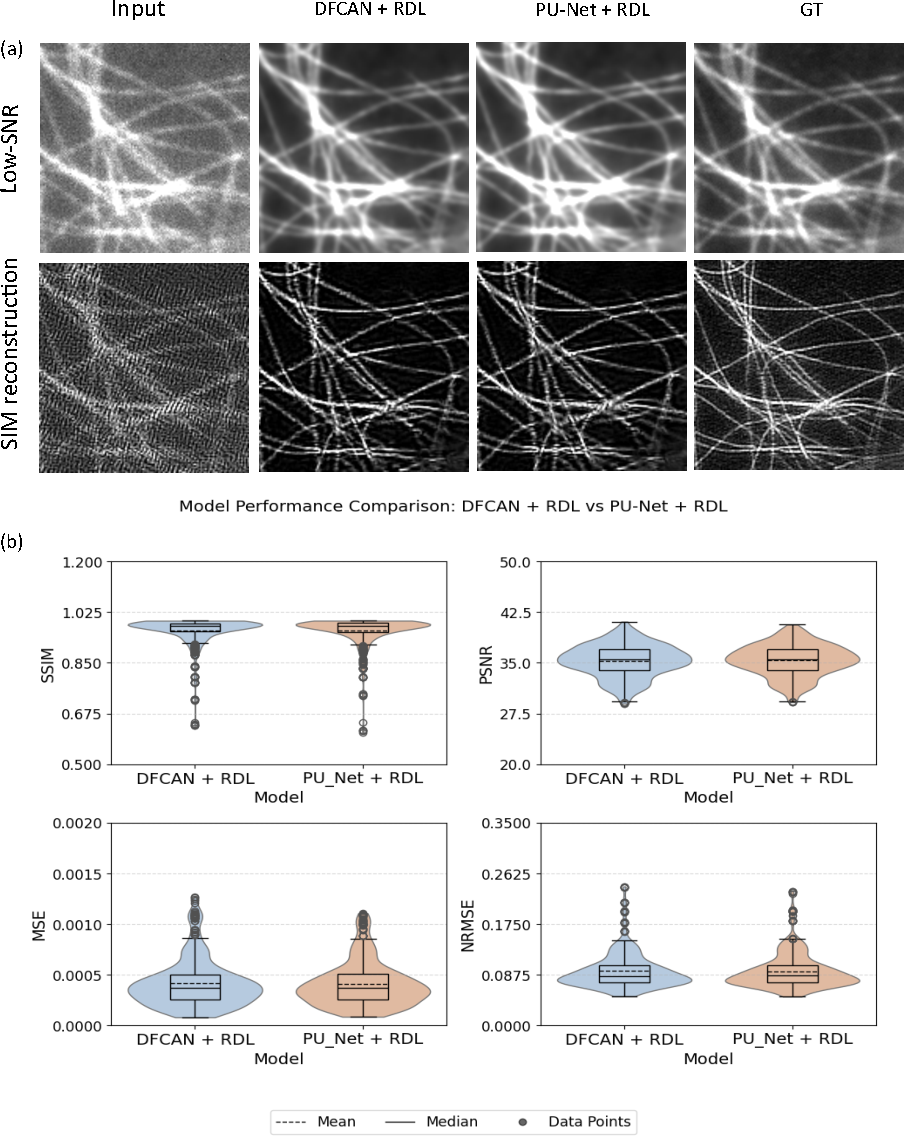
\includegraphics[width=\linewidth]{MT-02_DN-Compariosin_complete.pdf}
	\slcaption{
		(a) Image reconstruction of Microtubules from low SNR data, from DFCAN + RDL and 
		PU-Net (9×3×3) + RDL approaches are illustrated along with the corosponding SIM reconstruction. (b) Comparison of evaluation metrics shows that, the both approaches has similar performance. 	}
	\label{fig:MT-02_DN-Compariosin}
\end{figure}

% for MT-04
\begin{figure}[H]
	\centering
	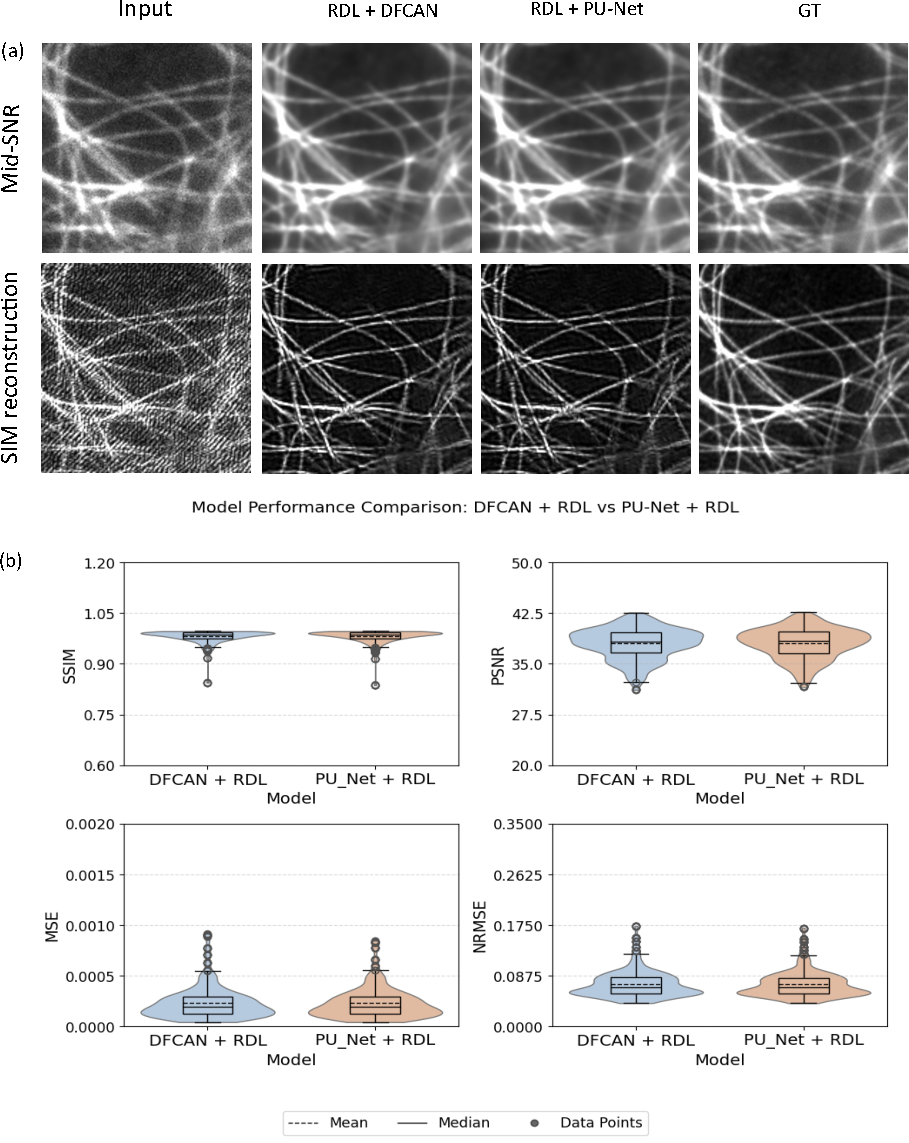
\includegraphics[width=\linewidth]{Mt-04_DN.pdf}
	\slcaption{(a) Image reconstruction of microtubules from mid SNR data, from DFCAN + RDL 
	and PU-Net (9×3×3) + RDL, along with the corresponding SIM reconstruction.

	(b) Comparison of evaluation metrics shows that, the both approaches has very similar performance. 	}
	\label{fig:Mt-04_DN}
\end{figure}



% for FA-04

\begin{figure}[H]
	\centering
	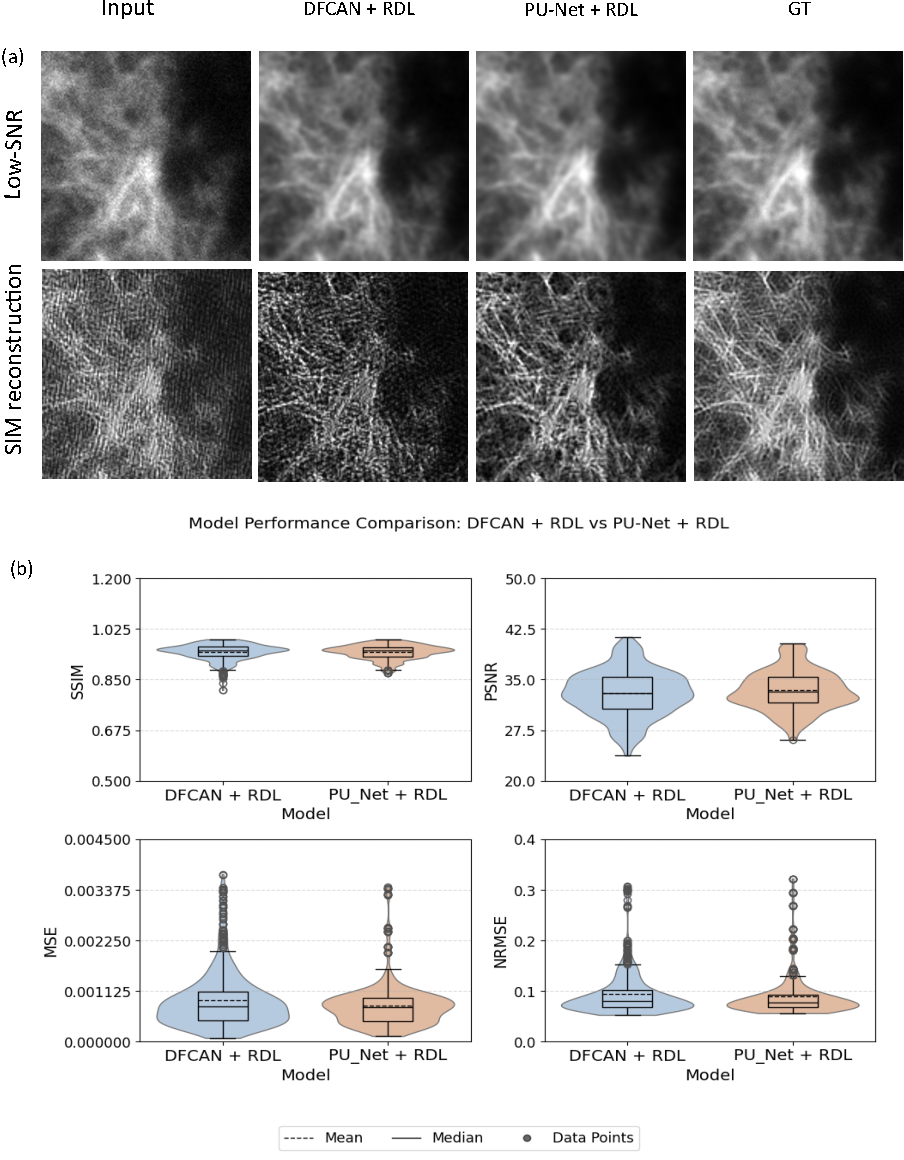
\includegraphics[width=\linewidth]{FA-DN_04.pdf}
	\slcaption{ (a) F-actin reconstructions from low-SNR raw data, alongside corresponding SIM images, are shown for both DFCAN + RDL and PU-Net (9×3×3) + RDL. 
	Despite fairSIM post-processing, both methods face challenges in resolving fine filament details due to high structural density and noise.
	(b) Evaluation metrics confirm that the two approaches achieve comparable performance.}
	\label{fig:FA-DN_04}
\end{figure}


% for FA-08

\begin{figure}[H]
	\centering
	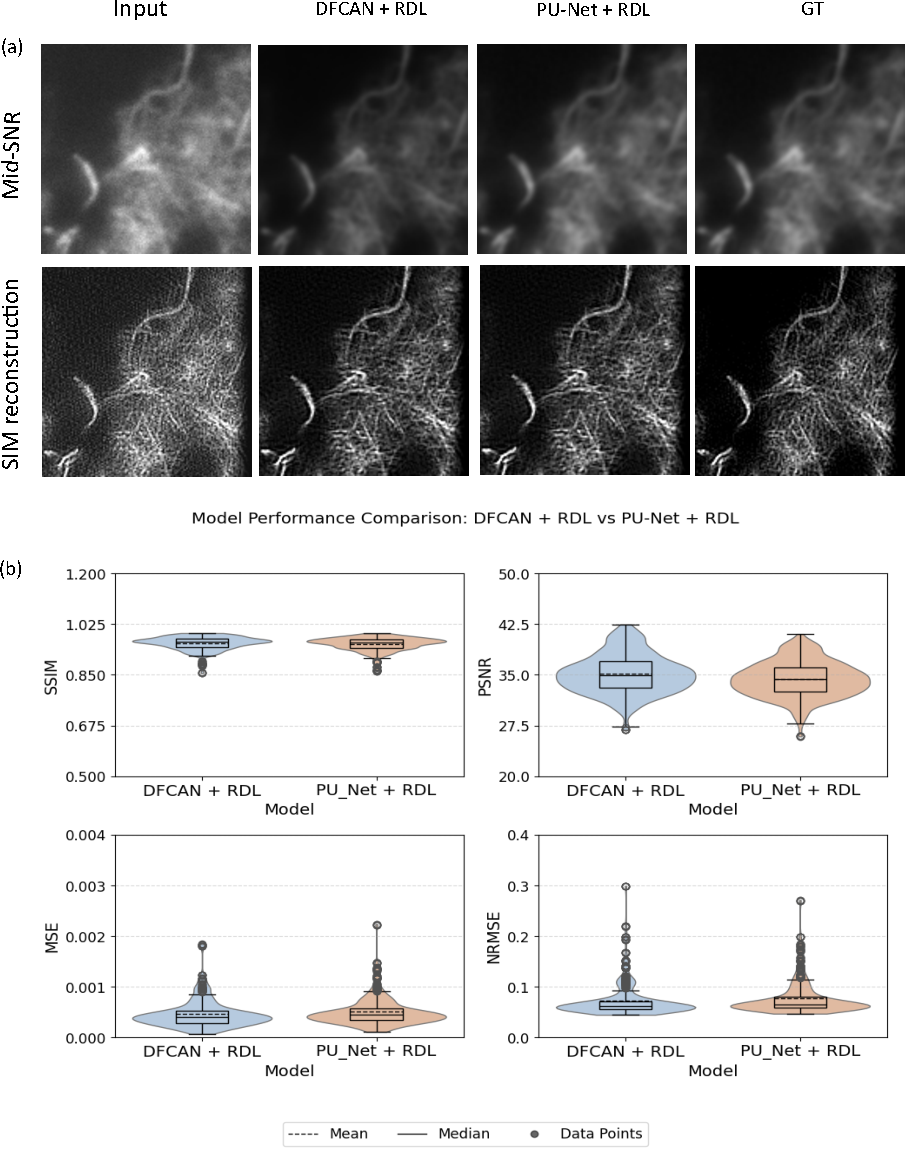
\includegraphics[width=\linewidth]{FN-08_DN_comparision.pdf}
	\slcaption{ (a) Image reconstruction of F-actin from mid-SNR noisy raw data, 
	along with the corresponding SIM reconstruction. The outputs from the DFCAN + RDL and PU-Net (9×3×3) + RDL approaches are presented.
	 In the post-processing with fairSIM, both methods reconstructs similar SIM reconstruction, proving the equivalance of the two approaches.
	  (b) Comparison of evaluation metrics indicates that both approaches exhibit comparable performance. }
	\label{fig:FN-08_DN_comparision}
\end{figure}




% for UNI_DATA_DN_LOW_SNR_FIX
\begin{figure}[H]
	\centering
	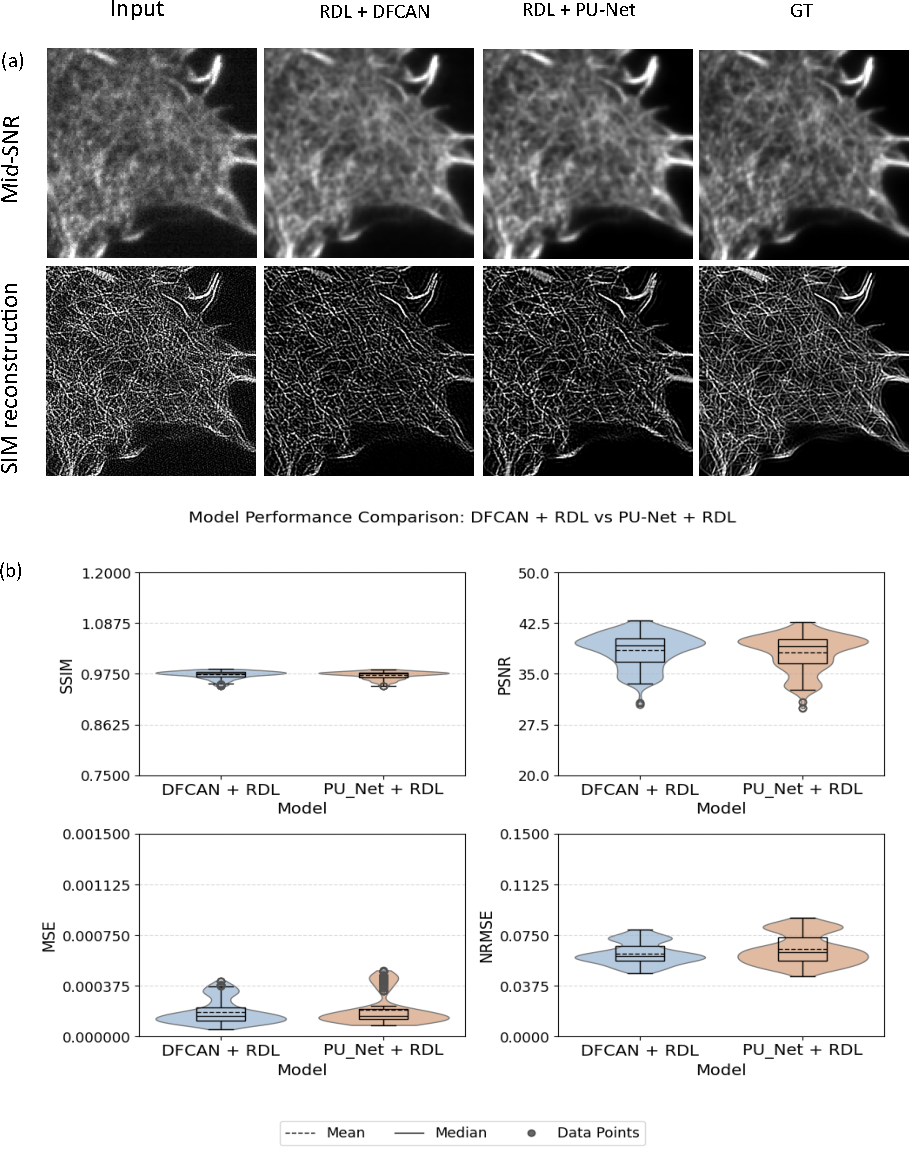
\includegraphics[width=\linewidth]{Uni_DATA_DN.pdf}
	\slcaption{ (a) Image reconstruction of F-actin from mid-SNR noisy raw data, 
	along with the corresponding SIM reconstruction. The outputs from the DFCAN + RDL and PU-Net (9×3×3) + RDL approaches are presented.
	 In the post-processing with fairSIM, both methods reconstructs similar SIM reconstruction, proving the equivalance of the two approaches.
	  (b) Comparison of evaluation metrics indicates that both approaches exhibit comparable performance. }
	\label{fig:Uni_DATA_DN}
\end{figure}





\chapter{Conclusion}

In this work, we investigated advanced deep learning architectures for enhancing Structured Illumination Microscopy (SIM) reconstruction,
 with a focus on denoising and resolution improvement under challenging low-SNR conditions. Through a comprehensive analysis of the Deep Fourier Channel Attention Network (DFCAN) 
 alongside various Projection Upsampling (PU) network architectures, our results indicate that while both approaches achieve comparable overall reconstruction performance,
  the PU-Net especially with the 9×3×3 kernel configuration demonstrates a notable advantage in capturing fine structural details in complex specimens such as microtubules and F-actin.




% Our findings emphasize the potential benefits of leveraging three-dimensional convolutional kernels to exploit spatio-temporal correlations inherent in multi-channel SIM data.
%  However, challenges remain in consistently resolving high-density and intricate features, suggesting that further improvements in network design, loss formulation, 
%  and training data diversity are critical for advancing performance.
\vspace{1cm}
\noindent
Our findings emphasize that, since the imaging is consistent in the 9 channels it images and concatenates as an image data, we can capturing spatial correlations across the channel
dimension by treating it as a Z dimension would add to the information not present in 2D kernel based models as they capture global cross-correlations across the channels 
 and may require laborious engineering based on Fourier approaches (like DFCAN) to retrieve that imformation. The approach of PU-Net on the other hand is much simpler and is intuitively
 ML centric in our use of 3D kernels to caputre the local information at scale reach the same performance level of DFCAN. 

\vspace{1cm}
\noindent
Futhermore, the complex stracture of F-actin and the high density of the data present significant challenges in accurately reconstructing 
fine filament details, what we see in all the experiments consistently. This indicates the need for larger tarining data as the complexity of the speciman increases.


\vspace{1cm}
\noindent
In summary, our work demonstrates the effectiveness of PU-Net in enhancing SIM reconstruction fidelity, gaining resolution and and documenting its effectiveness as substituting the DFCAN in the RDL-SIM pipeline.
% ''Future research will focus on refining the architecture and training strategies, including exploring alternative loss functions and more extensive data augmentation,
% to further enhance the reconstruction fidelity and generalization of these approaches in super-resolution microscopy.''

\clearpage
\chapter*{Acknowledgements}
%TODO A place to say thank you to everybody who helped you.

I would like to express my sincere gratitude to  Dr. rer. nat. Rainer Kurre and \\Dr. rer. nat. Varun Kapoor for their invaluable support and guidance throughout my research.
Their expertise and encouragement have been imperative in the completion of this thesis. 


\vspace{1cm}
\noindent
In addition, I would like to acknowledge the use of AI tools, such as ChatGPT and Claudia, which assisted me in debugging 
my code, paraphrasing and summarizing text to enhance my learning process during this work.



% Acronym definitions
%TODO Add acronym definitions produced by acronyms2glossary.py 




\glsaddall
\printglossaries
\printbibliography
\end{document}
